% demo.tex
%
% Enjoy, evolve, and share!
%
% Compile it as follows:
%	xelatex demo.tex
%   bibtex demo.aux
%   bibtex lop.aux (run this, only if you pass option 'lop' below)
%   xelatex demo.tex && xelatex demo.tex
%
% Alternatively, compile it using `make -i' (see the provided Makefile).
%
% Check file `diphdthesis.cls' for other configuration options.
%
\documentclass[inscr,ack,preface]{diphdthesis}

%\usepackage{graphicx}

%%%%%%%%%%%%%%%%%%%%%%%%%%%%%%%%%%%%%%%%%%%%%%%%%%%%%%%%%%%%%%%%%%%%%%%%%%%%%%%
%%%%%%%%%%%%%%%%%%%% User-specific package inclusions %%%%%%%%%%%%%%%%%%%%%%%%%
%%%%%%%%%%%%%%%%%%%%%%%%%%%%%%%%%%%%%%%%%%%%%%%%%%%%%%%%%%%%%%%%%%%%%%%%%%%%%%%
\usepackage{booktabs}
\usepackage{hyperref}
\hypersetup{
    unicode=true,                     % non-Latin characters in bookmarks
    pdffitwindow=true,                % page fit to window when opened
    pdfnewwindow=true,                % links in new window
    pdfkeywords={},                   % list of keywords
    colorlinks=true,                  % false: boxed links; true: colored links
    linkcolor=black,                  % color of internal links
    citecolor=black,                  % color of links to bibliography
    filecolor=black,                  % color of file links
    urlcolor=black,                   % color of external links
    pdftitle={},                      % title
    pdfauthor={},                     % author
    pdfsubject={}                     % subject of the document
}
%%%%%%%%%%%%%%%%%%%%%%%%%%%%%%%%%%%%%%%%%%%%%%%%%%%%%%%%%%%%%%%%%%%%%%%%%%%%%%%
%%%%%%%%%%%%%%%%%%%% User-specific package inclusions %%%%%%%%%%%%%%%%%%%%%%%%%
%%%%%%%%%%%%%%%%%%%%%%%%%%%%%%%%%%%%%%%%%%%%%%%%%%%%%%%%%%%%%%%%%%%%%%%%%%%%%%%


%%%%%%%%%%%%%%%%%%%%%%%%%%%%%%%%%%%%%%%%%%%%%%%%%%%%%%%%%%%%%%%%%%%%%%%%%%%%%%%
%%%%%%%%%%%%%%%%%%%%%% User-specific configuration %%%%%%%%%%%%%%%%%%%%%%%%%%%%
%%%%%%%%%%%%%%%%%%%%%%%%%%%%%%%%%%%%%%%%%%%%%%%%%%%%%%%%%%%%%%%%%%%%%%%%%%%%%%%
%%%%%%%%%%%%%%%%%%%%%%%%%%%%%%%%%%%%%%%%%%%%%%%%%%%%%%%%%%%%%%%%%%%%%%%%%%%%%%%
%%%%%%%%%%%%%%%%%%%%%% User-specific configuration %%%%%%%%%%%%%%%%%%%%%%%%%%%%
%%%%%%%%%%%%%%%%%%%%%%%%%%%%%%%%%%%%%%%%%%%%%%%%%%%%%%%%%%%%%%%%%%%%%%%%%%%%%%%


%%%%%%%%%%%%%%%%%%%%%%%%%%%%%%%%%%%%%%%%%%%%%%%%%%%%%%%%%%%%%%%%%%%%%%%%%%%%%%%
%%%%%%%%%%%%%%%%%%%%%%%%%%% Required Metadata %%%%%%%%%%%%%%%%%%%%%%%%%%%%%%%%%
%%%%%%%%%%%%%%%%%%%%%%%%%%%%%%%%%%%%%%%%%%%%%%%%%%%%%%%%%%%%%%%%%%%%%%%%%%%%%%%
%
% First name, last name
%
\authorFirstGr{Ευαγγελία}
\authorFirstAbrGr{Ε.} % abbreviation of first name
\authorMiddleGr{Γ.}   % abbreviation of father's first name
\authorLastGr{Στειροπούλου}
\authorFirstEn{Evangelia}
\authorFirstAbrEn{E.}
\authorMiddleEn{G.}
\authorLastEn{Steiropoulou}

%
% The title of the thesis
%
\titleGr{Υλοποίηση Κβαντικού Μετασχηματισμού Fourier μέσω μεταβαλλόμενων κβαντικών κυκλωμάτων}
\titleEn{Implementing Quantum Fourier Transform via variational quantum circuits}

%
% Month followed by Year
%
\dateGr{ΙΟΥΛΙΟΣ 2023}
\dateEn{JULY 2023}


%
% Advisor info
%

\advisorGr{Δημήτριος Συβρίδης}
\advisorRankGr{Καθηγητής}
\advisorOrgGr{Τμήμα Πληροφορικής και Τηλεπικοινωνιών}
\advisorEn{Dimitrios Syvridis}
\advisorRankEn{Professor}
\advisorOrgEn{Department of Informatics and Telecommunications}

%
% Abstract, synopsis, inscription, ack, and preface pages.
%

% \usepackage{babel} % Load the babel package for multilingual support
\usepackage{ragged2e}

\abstractEn{
% \selectlanguage{English} % Set the language to English
\begin{justify}
    Variational quantum circuits are quantum circuits which contain gates with 
     adjustable parameters. Such circuits are already physically realizable in small scale and there is a wide
    range of possible applications for these promising structures. In this thesis, we develop the idea of tuning  a variational quantum circuit
    to simulate the important for quantum computing, operation of Quantum Fourier Transform.
    I use algebraic arguments, so called an ansatz, for reducing the depth of the variational quantum circuit 
    and I use different classical algorithms to optimize the parameters. The results of this thesis concerning 3-\acrshort{qubit} circuits can be possibly extended to 
    a higher number of \acrshort{qubit}s.
    \end{justify}
}

\abstractGr{    
% \selectlanguage{Greek} % Set the language to Greek
    \begin{justify}
        Τα μεταβαλλόμενα κβαντικά κυκλώματα είναι κυκλώματα που περιέχουν κβαντικές πύλες, με παραμέτρους που μεταβάλλονται κατά τη διάρκεια της εκτέλεσης. Τα συγκεκριμένα κυκλώματα είναι ήδη φυσικά εφαρμόσιμα σε μικρή κλίμακα και υπάρχει μια ευρεία γκάμα δυνατών εφαρμογών για αυτά. Σε αυτήν την εργασία, αναπτύσσουμε την ιδέα της υλοποί-
        ησης ενός μεταβαλλόμενου κβαντικού κυκλώματος για να προσομοιώσουμε μια σημαντική για τον κβαντικό υπολογισμό λειτουργία, τον Κβαντικό Μετασχηματισμό Fourier (Quantum Fourier Transform). Χρησιμοποιού-
        με αλγεβρικά δεδομένα, έναν επονομαζόμενο ανσάτζ (ansatz) για να μειώσουμε το βάθος του ποιοτικού κβαντικού κυκλώματος και χρησιμοποιούμε διάφορους κλασικούς αλγορίθμους για να βελτιστοποιήσουμε τις παρα-
        μέτρους. Τα αποτελέσματα αυτής της εργασίας σχετικά με τα κυκλώματα τριών \acrshort{qubit} μπορούν να επεκταθούν πιθανώς σε περισσότερα \acrshort{qubit}s. 
    \end{justify}
}
\acksEn{}
\prefaceEn{}

\inscriptionEn{Στην οικογένειά μου}

% %
% % Subject area and keywords
% %
\subjectAreaGr{Κβαντική υπολογιστική}
\subjectAreaEn{Quantum computing}
\keywordsGr{κβαντικά κυκλώματα, κβαντικός μετασχηματισμός Fourier, αλγόριθμοι βελτιστοποίησης}
\keywordsEn{quantum circuits, quantum Fourier transform, optimization algorithms}

%
% Set the .bib file containing your paper publications (leave the extension out)
%
% This is optional, but it should be specified when option 'lop' is passed to
% the document class.
%
% Then, inside the document environment, you may use the command '\nocitelop' to
% site your papers, as you would traditionally do with the commands '\cite' or
% '\nocite'.
%
% The papers are printed in reverse chronological order.
%
%\lopfile{mypapers/pubs}
%%%%%%%%%%%%%%%%%%%%%%%%%%%%%%%%%%%%%%%%%%%%%%%%%%%%%%%%%%%%%%%%%%%%%%%%%%%%%%%
%%%%%%%%%%%%%%%%%%%%%%%%%%% Required Metadata %%%%%%%%%%%%%%%%%%%%%%%%%%%%%%%%%
%%%%%%%%%%%%%%%%%%%%%%%%%%%%%%%%%%%%%%%%%%%%%%%%%%%%%%%%%%%%%%%%%%%%%%%%%%%%%%%

\usepackage{enumitem}
\usepackage{amsmath}
\usepackage{pdfpages}
\usepackage{caption}
\usepackage{amsfonts}
\usepackage{glossaries}
\usepackage{float}
\usepackage{booktabs}
\usepackage{fontspec}

\makeglossaries
\renewcommand{\glossaryname}{ABBREVATIONS - ACRONYMS} % Change the title to "Abbreviations"

\captionsetup{labelfont=bf, textfont=bf}

\newacronym{qubit}{qubit}{quantum bit}
\newacronym{vqa}{VQA}{Variational Quantum Algorithms}
\newacronym{vqc}{VQC}{Variational Quantum Circuits}
\newacronym{qft}{QFT}{Quantum Fourier Transform}
\newacronym{rsa}{RSA}{Rivest–Shamir–Adleman}
\newacronym{cnot}{CNOT}{controlled-NOT}
\newacronym{ghz}{GHZ}{Greenberger-Horne-Zeilinger}

\begin{document}

\frontmatter

% \selectlanguage{English} % Set the language to English

% site my papers
%\nocitelop{}


\mainmatter

% add main chapters (should be given in capital letters)
\chapter{INTRODUCTION}

In the era where quantum technologies become a reality, it is useful to seek into the 
new opportunities offered to a computer scientist. While the well-known quantum algorithms
offering exponential advantage over classical ones are out of the scope of realization because of
the requiring  quantum resources, a new sort of algorithms  has emerged
which is suitable for the current experimental status and which is still promising for exhibiting a quantum advantage.
These algorithms,  the so called \acrfull{vqa} are hybrid requiring low-depth \acrfull{vqc} but also a classical optimization loop. \acrshort{vqa}s are addressing different problems, using different ansatzs, but their underlined structure
is the same, resembling the one of a classical neural network where the weights/parameters are trained via a gradient descent method. 

In this work, inspired from the work "Quantum Assisted Quantum Compiling"\cite{paper} we aim to train of a \acrshort{vqc} to simulate approximately 
the effect of a circuit implementing \acrfull{qft}. We first build an ansatz in order to avoid to work with \acrshort{vqc} of random structure and to  reduce the depth. Then we show that with this ansatz a relatively low-depth circuit is able to approximate the \acrshort{qft} on three \acrshort{qubit}s. This result if it is extensible to a higher number of \acrshort{qubit}s can be of importance, since \acrshort{qft} is the basic block for Shor's quantum algorithm which threatens security of \acrshort{rsa} cryptographic scheme.
We also study another important aspect for this method and of \acrshort{vqa} algorithms in general, that is the appropriate choice
of the classical optimization algorithm. We see that for the case under study a gradient descent method performs better
than a stochastic one.
 
 In what follows, we first provide the basic elements of a quantum circuit. Then we give some information on
the operation of a \acrshort{qft} and provide the initial circuit representation of it for $3$ \acrshort{qubit}s. In chapter~\ref{VQA} an overview about
\acrshort{vqc}s and \acrshort{vqa}s is provided, while finally in chapter~\ref{results} we present our results.

\chapter{THE BASIC ELEMENTS OF QUANTUM CIRCUITS}

Quantum circuits are a fundamental concept in quantum computation, similar to classical circuits. They consist of a sequence of quantum gates, measurements, \acrshort{qubit} initializations, and other actions that enable quantum computation. \cite{niel}. It's important to note that quantum circuits differ from classical circuits as they operate on \acrshort{qubit}s, which can exist in superpositions of states. This allows for the exploration of multiple possibilities simultaneously, which is a key advantage of quantum computation. 

\section{Qubit}

The first thing we need to define, is the basic quantum computational unit, the \acrshort{qubit} that is the the short for quantum bit. 
 While classical bits can only have two possible states (0 or 1), \acrshort{qubit}s can exist in a superposition of both states simultaneously. This means that a \acrshort{qubit} can be in a linear combination of the 0 and 1 states. A \acrshort{qubit} is a two-level quantum system, with the two basis \acrshort{qubit} states usually represented as $\vert0\rangle$ and $\vert1\rangle$. A \acrshort{qubit} can be in state $\vert0\rangle$, $\vert1\rangle$, or in a superposition of both states as $\cos \theta\vert0\rangle+\sin\theta e^{i\phi} \vert1\rangle$. The superposition property allows a quantum computer to be in multiple states at once, which leads to the exponential growth of possible states as the number of \acrshort{qubit}s increases \cite{qubit}. It is also convenient for calculations to represent 
 \acrshort{qubit}  as vectors
 \begin{center}
 \Large
 $\vert0\rangle = 
    \begin{bmatrix}
    1 \\
    0 \\
    \end{bmatrix}$
\end{center}
\normalsize
and \\
\begin{center}
\Large
$\vert1\rangle = 
\begin{bmatrix}
0 \\
1 \\
\end{bmatrix}$
\end{center}
\normalsize
To understand the concept of a \acrshort{qubit}, it's helpful to think about examples from the physical world. A simple analogy, is polarized light. Polarized light can be thought of as a \acrshort{qubit} because it exist in two mutually exclusive/orthogonal states: vertically polarized or horizontally polarized. However, if in a general state a single measurement will give both two answers, each one with a partial weight. In contrast, a \acrshort{qubit} can be asked many different questions, but each question can only have one of two possible outcomes \cite{polarized}.

In practice, \acrshort{qubit}s are realized using various physical systems, such as the spin of an electron or the polarization of a photon. The spin of an electron is a common example of a \acrshort{qubit}. The two levels of the electron's spin can be taken as spin up and spin down, which correspond to the 0 and 1 states of a \acrshort{qubit} \cite{electron}. Similarly, the polarization of a single photon can be used to represent the 0 and 1 states of a \acrshort{qubit}.

It's important to note that \acrshort{qubit}s are not limited to two-level systems. Qudits and qutrits are terms used to describe quantum systems with more than two levels. A qudit is a unit of quantum information that can be realized in suitable d-level quantum systems, where d is an integer \cite{qudit}.

The behavior of \acrshort{qubit}s is governed by the principles of quantum mechanics, such as superposition and entanglement. Superposition allows \acrshort{qubit}s to exist in multiple states simultaneously, while entanglement enables the correlation of \acrshort{qubit}s even when they are physically separated. These properties are fundamental to quantum computing and enable the potential for exponential speedup in certain computational tasks compared to classical computers.

We can use the Bloch sphere to represent the state of a single \acrshort{qubit}, see Figure~\ref{fig:enter-label}. Any
state in a quantum computation can be represented as a vector that begins at
the origin and terminates on the surface of the unit Bloch sphere. By applying
unitary operators to the state vectors, we can move the state around the surface of the sphere.
We take as convention that the poles of the sphere are $\vert0\rangle$ on the top and $\vert1\rangle$ on the bottom \cite{hidary}.
We can also represent superposition states such as 
\Large $\frac{\lvert 0 \rangle + \lvert 1 \rangle}{\sqrt{2}}$ 
\normalsize that lies along the X axis  on Figure~\ref{fig:enter-label}.
\begin{figure}[ht]
    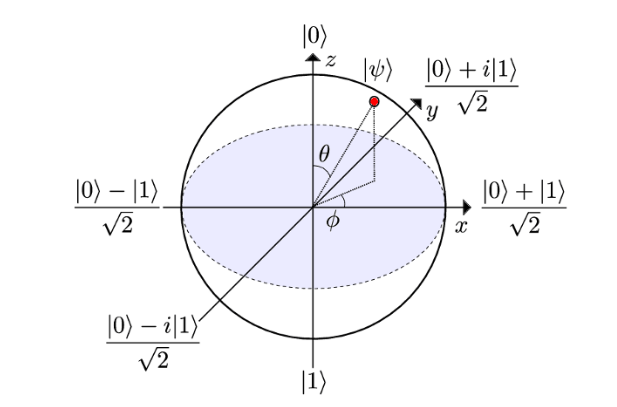
\includegraphics[width=0.9\textwidth]{bloch.png}
    \caption{The Bloch Sphere}
    \label{fig:enter-label}
\end{figure}

\cite{kockum2014quantum}


\section{Quantum Gates}

The building blocks of quantum circuits, are the quantum gates. They are operations performed on \acrshort{qubit}s, such as rotations, flips, and entanging gates. Quantum gates can manipulate the quantum state of the \acrshort{qubit}s, enabling various computations and transformations. Quantum logic gates can be derived from classical logic gates, but the Hilbert-space structure of \acrshort{qubit}s allows for an infinite number quantum gates that are not induced by classical gates.

Quantum gates are described as unitary operators, represented by unitary matrices relative to some basis. The action of a quantum gate on a \acrshort{qubit} can be represented by a matrix multiplication of the gate's unitary matrix with the \acrshort{qubit}'s state vector. Hermitian gates, such as the Pauli gates, Hadamard gate, \acrshort{cnot} gate, SWAP gate, and Toffoli gate, are examples of gates that are both Hermitian and unitary.

The representation of Pauli gates and other important gates as matrices is the following, \cite{niel},:
\begin{itemize}
    \item Pauli-X gate (NOT gate):
    \begin{center}
    \Large
        $X = \sigma_x = \sigma_1 = 
        \begin{bmatrix}
            0 & 1 \\
            1 & 0 \\
        \end{bmatrix}$
    \end{center}
    \normalsize
    \item Pauli-Y gate:
    \begin{center}
    \Large
        $Y = \sigma_y = \sigma_2 = 
        \begin{bmatrix}
            0 & -i \\
            i & 0 \\
        \end{bmatrix}$
    \end{center}
    \normalsize
    \item Pauli-Z gate:
    \begin{center}
    \Large
        $Z = \sigma_z = \sigma_3 = 
        \begin{bmatrix}
            1 & 0 \\
            0 & -1 \\
        \end{bmatrix}$
    \end{center}
    \normalsize
    \item Pauli-I gate (identity gate):
    \begin{center}
    \Large
        $I =  \sigma_4 = 
        \begin{bmatrix}
            1 & 0 \\
            0 & 1 \\
        \end{bmatrix}$
    \end{center}
    \item Hadamard gate:
    \begin{center}
    \Large
        $H = \frac{1}{\sqrt{2}}\begin{bmatrix}
            1 & 1 \\
            1 & -1 \\
            \end{bmatrix}$
    \end{center}
    
\end{itemize}
We will be mentioning these gates a lot as we move on in this project.
Lets study an example of the X-gate matrix applied to a \acrshort{qubit} in state $|0\rangle$:
\Large
\begin{center}
$X|0\rangle = \begin{bmatrix}
0 & 1 \\
1 & 0 \\
\end{bmatrix}
\begin{bmatrix}
1 \\
0 \\
\end{bmatrix} = 
\begin{bmatrix}
0 \\
1 \\
\end{bmatrix} = |1\rangle$

\end{center}
\normalsize

Unlike classical logic gates, quantum gates are reversible. This means that the input state can be recovered from the output state by applying the same gate in reverse. Reversibility is a fundamental property of quantum gates and is a consequence of the unitary nature of quantum operations. Reversibility allows for the efficient simulation of classical computation using quantum circuits.

To prove it, we will apply the X-gate on the previous result, and we will notice that the initial input is the initial state:

\Large
\begin{center}
$X|1\rangle = \begin{bmatrix}
0 & 1 \\
1 & 0 \\
\end{bmatrix}
\begin{bmatrix}
0 \\
1 \\
\end{bmatrix} = 
\begin{bmatrix}
1 \\
0 \\
\end{bmatrix} = |0\rangle$

\end{center}
\normalsize

\subsection{Single Qubit Gates}

In the field of quantum computing, single \acrshort{qubit} gates and 2-\acrshort{qubit} gates play a crucial role in manipulating and transforming the quantum states of \acrshort{qubit}s. These gates are used to perform operations on individual \acrshort{qubit}s and multiple \acrshort{qubit}s, respectively.

Starting with single \acrshort{qubit} gates, they act on individual \acrshort{qubit}s and can be used to change their state or perform specific operations. Some commonly used single \acrshort{qubit} gates, are the ones we mentioned before, the Pauli-X gate (bit-flip), Pauli-Y gate (bit and phase flip), Pauli-Z gate (phase flip), Hadamard gate (superposition), and the identity gate. Each of these gates is represented by a unitary matrix and operates on the state vector of a single \acrshort{qubit}. We showed their application above. Single \acrshort{qubit} gates can be physically realized using techniques such as laser pulses or microwave pulses to manipulate the state of individual \acrshort{qubit}s \cite{microwave}.

\subsection{2-Qubit and 3-qubit Gates}
Moving on to 2-\acrshort{qubit} gates, these act on two \acrshort{qubit}s simultaneously inducing interaction between them. The \acrfull{cnot} gate is a commonly used 2-\acrshort{qubit} gate. It performs a controlled operation where the second \acrshort{qubit} (target \acrshort{qubit}) is flipped if and only if the first \acrshort{qubit} (control \acrshort{qubit}) is in the state $|1\rangle$. In matrix representation in the computational basis, \acrfull{cnot} gate writes as
    \begin{center}
    \Large
    $CNOT = 
        \begin{bmatrix}
            1 & 0 & 0 & 0 \\
            0 & 1 & 0 & 0 \\
            0 & 0 & 0 & 1 \\
            0 & 0 & 1 & 0 \\
        \end{bmatrix}$
    \end{center}
\normalsize

\begin{center}
\Large
$CNOT(|0\rangle\otimes|0\rangle) &=\begin{bmatrix} 1 & 0 & 0 & 0 \\ 0 & 1 & 0 & 0 \\ 0 & 0 & 0 & 1 \\ 0 & 0 & 1 & 0 \end{bmatrix} \begin{bmatrix} 1 \\ 0 \\ 0 \\ 0 \end{bmatrix}
&= \begin{bmatrix} 1 \\ 0 \\ 0 \\ 0 \end{bmatrix} = |00\rangle$
\end{center}
\normalsize
Lets apply the \acrshort{cnot} gate on \Large $|10\rangle$: \\
\begin{center}
\Large
$CNOT(|1\rangle\otimes|0\rangle)) = \begin{bmatrix}
1 & 0 & 0 & 0 \\
0 & 1 & 0 & 0 \\
0 & 0 & 0 & 1 \\
0 & 0 & 1 & 0 \\
\end{bmatrix}
\begin{bmatrix}
0 \\
0 \\
1 \\
0 \\
\end{bmatrix}
= \begin{bmatrix}
0 \\
0 \\
0 \\
1 \\
\end{bmatrix}
= |11\rangle$
\end{center}
\normalsize
As we can see, now that the control \acrshort{qubit} is $|1\rangle$ the target \acrshort{qubit} becomes from $|0\rangle$, $|1\rangle$.
\\
Concerning 3-\acrshort{qubit} gates, the extension of \acrfull{cnot} gate is the Toffoli gate, which is a reversible gate that performs a NOT operation on the target \acrshort{qubit} if both control \acrshort{qubit}s are in the state $|1\rangle$. Similar to  2-\acrshort{qubit} gates, 3-\acrshort{qubit} gates can be physically implemented using techniques  controlling interactions between \acrshort{qubit}s. Providing a couple of examples:
\begin{itemize}
\item Toffoli gate:
    \begin{center}
    \Large
\[\begin{bmatrix}
        1 & 0 & 0 & 0 & 0 & 0 & 0 & 0 \\
        0 & 1 & 0 & 0 & 0 & 0 & 0 & 0 \\
        0 & 0 & 1 & 0 & 0 & 0 & 0 & 0 \\
        0 & 0 & 0 & 1 & 0 & 0 & 0 & 0 \\
        0 & 0 & 0 & 0 & 1 & 0 & 0 & 0 \\
        0 & 0 & 0 & 0 & 0 & 1 & 0 & 0 \\
        0 & 0 & 0 & 0 & 0 & 0 & 0 & 1 \\
        0 & 0 & 0 & 0 & 0 & 0 & 1 & 0 \\
    \end{bmatrix}\]    
    \normalsize
    \end{center}
    \item Fredkin gate(controlled-swap):
    \begin{center}

\[    \Large\begin{bmatrix}
        1 & 0 & 0 & 0 & 0 & 0 & 0 & 0 \\
        0 & 1 & 0 & 0 & 0 & 0 & 0 & 0 \\
        0 & 0 & 1 & 0 & 0 & 0 & 0 & 0 \\
        0 & 0 & 0 & 1 & 0 & 0 & 0 & 0 \\
        0 & 0 & 0 & 0 & 1 & 0 & 0 & 0 \\
        0 & 0 & 0 & 0 & 0 & 0 & 1 & 0 \\
        0 & 0 & 0 & 0 & 0 & 1 & 0 & 0 \\
        0 & 0 & 0 & 0 & 0 & 0 & 0 & 1 \\
    \end{bmatrix}\]    
\normalsize
\end{center}
\end{itemize}

In the context of quantum computing, gates can be combined in series or in parallel to create more complex operations and circuits. Series combinations of gates involve applying one gate after another, while parallel combinations involve applying gates simultaneously to different \acrshort{qubit}s. The order of gates in a circuit diagram is reversed to the the multiplication procedure written in formulas. 

To sum it up, single \acrshort{qubit} gates, 2 and 3 \acrshort{qubit} gates are fundamental components in quantum computing. They are used to manipulate and transform the quantum states of \acrshort{qubit}s, enabling the implementation of various quantum algorithms and protocols. Single \acrshort{qubit} gates act on individual \acrshort{qubit}s, while 2 \acrshort{qubit} gates allow for interactions between pairs of \acrshort{qubit}s. These gates can be combined to create more complex operations and circuits, as we will see later. 

\subsection{Variational Gates}

Another category of gates, is what we call variational gates. These are  gates with trainable/free parameters within, which are used in variational circuits. In this project, I use both single, and 2-\acrshort{qubit} variational gates.
Since, my results concern 3-qubit circuits I will explain here, via the generators of the $su(8)$ algebra of 3 qubits, the variational gates that I will use later. One can create the $64$ generators of the group by taking 
 the Kronecker product of 4 single \acrshort{qubit} operators (X-gate, Y-gate, Z-gate and Identity gate). This way we can have up to 64 different generators $\hat{g}_{i,j,k}$ with $i,j,k=1,\ldots 4$. For example a generator can be $\hat{g}_{1,4,4}=\hat{X}\otimes 1\otimes1$ or $\hat{g}_{1,4,2}=\hat{X}\otimes 1\otimes \hat{Y}$ etc. Note that 1 represents the Identity matrix. 
 The variational gates of the circuit are constructed by exponentiation of
 this generator $\hat{g}_{j,j,k}$ multiplied by a parameter $x$, as
 \[\hat{R}_{\hat{g}_{j,j,k}(x)=e^{ix \hat{g}_{j,j,k}}\]
 In geometric space such gates $\hat{R}_{\hat{g}_{j,j,k}}(x)$  perform a rotation around the axis that is defined by the generator $\hat{g}_{j,j,k}$ while the rotation angle  is proportional to the parameter x. Further information on this matter, is provided in \autoref{chap:qft_vqc}. Let me provide some examples, the varitional gate
\begin{center}
\begin{equation}  
\Large\hat{R}_{\hat{X}\otimes 1\otimes1}(x)=e^{i x \hat{X}\otimes 1\otimes1}\label{eq:2.1}
\end{equation}
\end{center}
is a single qubits variational gate while
\begin{center}
\begin{equation} 
\Large\hat{R}_{\hat{X}\otimes 1\otimes \hat{Y}}(x)=e^{i x \hat{X}\otimes 1\otimes\hat{Y}}\label{eq:2.2}
\end{equation}
\end{center} 
is a 2-qubit gate acting on the first and third qubit.

Let me here clarify how exponetniation and Kronecker product works using the examples in Eqs.(\ref{eq:2.1})-(\ref{eq:2.2}). Knowing that
\[
X = \begin{bmatrix}
0 & 1 \\
1 & 0 \\
\end{bmatrix},
\quad
I = \begin{bmatrix}
1 & 0 \\
0 & 1 \\
\end{bmatrix}
\]
then Kronecker product is computed as follows:\\
\begin{alignat*}{2}
X \otimes I &= \begin{bmatrix}
    0 & 1 \\
    1 & 0 \\
\end{bmatrix} \otimes \begin{bmatrix}
    1 & 0 \\
    0 & 1 \\
\end{bmatrix} &\quad&
= \begin{bmatrix}
    0 & 0 & 1 & 0 \\
    0 & 0 & 0 & 1 \\
    1 & 0 & 0 & 0 \\
    0 & 1 & 0 & 0 \\
\end{bmatrix}
\end{alignat*}

\begin{alignat*}{2}
X \otimes I \otimes I &= \begin{bmatrix}
    0 & 0 & 1 & 0 \\
    0 & 0 & 0 & 1 \\
    1 & 0 & 0 & 0 \\
    0 & 1 & 0 & 0 \\
\end{bmatrix} \otimes \begin{bmatrix}
    1 & 0 \\
    0 & 1 \\
\end{bmatrix} &\quad&
= \begin{bmatrix}
    0 & 0 & 0 & 0 & 1 & 0 & 0 & 0 \\
    0 & 0 & 0 & 0 & 0 & 1 & 0 & 0 \\
    0 & 0 & 0 & 0 & 0 & 0 & 1 & 0 \\
    0 & 0 & 0 & 0 & 0 & 0 & 0 & 1 \\
    1 & 0 & 0 & 0 & 0 & 0 & 0 & 0 \\
    0 & 1 & 0 & 0 & 0 & 0 & 0 & 0 \\
    0 & 0 & 1 & 0 & 0 & 0 & 0 & 0 \\
    0 & 0 & 0 & 1 & 0 & 0 & 0 & 0 \\
\end{bmatrix}
\end{alignat*}
The corresponding single-qubit variational gate can be computed by the formula
\[\Large
\hat{R}_{\hat{X}\otimes 1\otimes1}(x) = e^{i x \hat{X}\otimes 1\otimes1} = \exp \left( i x \begin{bmatrix}
    0 & 0 & 0 & 0 & 1 & 0 & 0 & 0 \\
    0 & 0 & 0 & 0 & 0 & 1 & 0 & 0 \\
    0 & 0 & 0 & 0 & 0 & 0 & 1 & 0 \\
    0 & 0 & 0 & 0 & 0 & 0 & 0 & 1 \\
    1 & 0 & 0 & 0 & 0 & 0 & 0 & 0 \\
    0 & 1 & 0 & 0 & 0 & 0 & 0 & 0 \\
    0 & 0 & 1 & 0 & 0 & 0 & 0 & 0 \\
    0 & 0 & 0 & 1 & 0 & 0 & 0 & 0 \\
\end{bmatrix}\right)\]
\normalsize  
using spectral theorem or Taylor expansion.

Similarly for the equation {\ref{eq:2.2}} the generator is the Kronecker product of a X-Pauli gate, with the Identity gate, and the Y-Pauli gate. 
Following the same process as before, we can write this 2-qubit variational gate as 
\[\Large\hat{R}_{\hat{X}\otimes 1\otimes \hat{Y}}(x)=e^{  i x \hat{X}\otimes 1\otimes\hat{Y}} = \exp \left(i x \begin{bmatrix} 0 & 0 & 0 & 0 & 0 & -i & 0 & 0 \\ 0 & 0 & 0 & 0 & i & 0 & 0 & 0 \\ 0 & 0 & 0 & 0 & 0 & 0 & 0 & -i \\ 0 & 0 & 0 & 0 & 0 & 0 & i & 0 \\ 0 & -i & 0 & 0 & 0 & 0 & 0 & 0 \\ i & 0 & 0 & 0 & 0 & 0 & 0 & 0 \\ 0 & 0 & 0 & -i & 0 & 0 & 0 & 0 \\ 0 & 0 & i & 0 & 0 & 0 & 0 & 0  \end{bmatrix} \right)\] \normalsize

\section{Measurements}

Measurement is another important aspect of quantum circuits. Measurements are used to extract information from \acrshort{qubit}s. They collapse the quantum state of a \acrshort{qubit} to one of its basis states, and the measurement result is a classical value that can be used in classical computations. It's important to note that measurement in quantum mechanics is probabilistic, and the outcome of a measurement cannot be predicted with certainty but the probabilities can be inferred if the state of qubits is known.

\section{Quantum circuits}

Now using a combination of the gates mentioned before, we will create a circuit. Specifically, we will provide the a circuit, that entangles 3 \acrshort{qubit}s. As we can see, the circuit is composed of a Hadamard gate($H$), followed by two $\acrshort{cnot}$ gates, and lastly the measurements of the 3 \acrshort{qubit}s. \cite{ibm}
\begin{figure}[ht]
    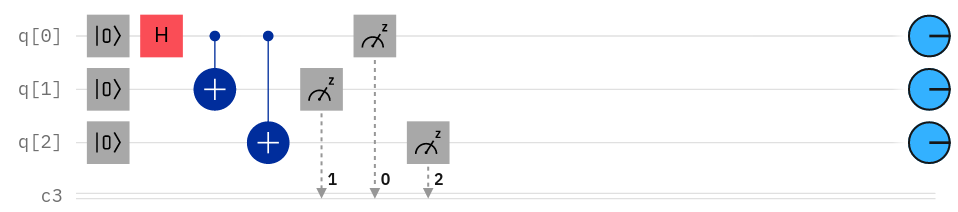
\includegraphics[width=1\textwidth]{ghz.png}
    \caption{GHZ states circuit}
    \label{fig:enter-label}
\end{figure}

\acrshort{ghz} states are named after Greenberger, Horne, and Zeilinger, who were the first to study them in 1989. \acrshort{ghz} states are also known as “Schrödinger cat states” or just “cat states.” \cite{ghz_ibm}

\chapter{QUANTUM FOURIER TRANSFORM (QFT)}

One of the most useful ways of solving a problem in mathematics or computer science is to transform it into some other problem for which a solution is known.  A great discovery of quantum computation has been that some such transformations can be computed much faster on a quantum computer than on a classical computer, a discovery which has enabled the construction of fast algorithms for quantum computers.

The Quantum Fourier Transform is a reversible transformation that operates on \acrshort{qubit}s and is used to convert a quantum state from the computational basis to the Fourier basis. It is implemented using a series of unitary gates, such as the Hadamard gate and the controlled phase shift gate \cite{niel}. The \acrshort{qft} is particularly powerful when combined with other algorithms, as it can be used to measure the period of a function, which is essential for cracking the \acrshort{rsa} algorithm.

The algorithm implements a Discrete Fourier transform on the values
of the amplitudes. As a reminder, the classical version of the Fourier transform takes as input a vector of complex numbers \(x_0, x_1, \ldots, x_{N-1}\), where the length N of the vector is a fixed parameter. It outputs the transformed data, a vector of complex numbers \(y_0, y_1, \ldots, y_{N-1}\) , defined by
\begin{equation}
    y_k \equiv \frac{1}{\sqrt{N}} \sum_{j=0}^{N-1} x_j e^{\frac{2\pi ijk}{N}}\
\end{equation}

The Quantum Fourier transform is exactly the same transformation, although the
conventional notation for the quantum Fourier transform is somewhat different. The
quantum Fourier transform on an orthonormal basis \(|0\rangle, \ldots, |N − 1\rangle\) is defined to be a linear operator with the following action on the basis states
\begin{equation}
    |j\rangle  \rightarrow \frac{1}{\sqrt{N}} \sum_{j=0}^{N-1} x_j e^{\frac{2\pi ijk}{N}} |k\rangle\
\end{equation}

Equivalently, the action on an arbitrary state may be written
\begin{equation}
        \sum_{j=0}^{N-1} x_j |j\rangle  \rightarrow \sum_{k=0}^{N-1} y_k|k\rangle\
\end{equation}   
where the amplitudes $y_k$ are the discrete Fourier transform of the amplitudes $x_j$ \cite{niel}. In other words, the quantum Fourier transform implements a discrete Fourier transform on the values
of the amplitudes of an input state. This transformation is a unitary transformation, and thus can be implemented via a circuit of a quantum computer \cite{supervised}.


\section{QFT on 3 qubits}
QFT operation has been proposed together with a circuit implementation where the number of gates increases approximately quadratically  with the number of qubits.
On the other hand this circuit, as we are going to show, contains Controlled-Phase gates whose design and implementation are hard in general.
 The \acrshort{qft} with 3 \acrshort{qubit}s requiring 6 gates, see Figure~\ref{fig:enter-label}, is the first non-trivial case, and for this reason
 we have chosen to work with.

\begin{figure}[ht]
\begin{center}
    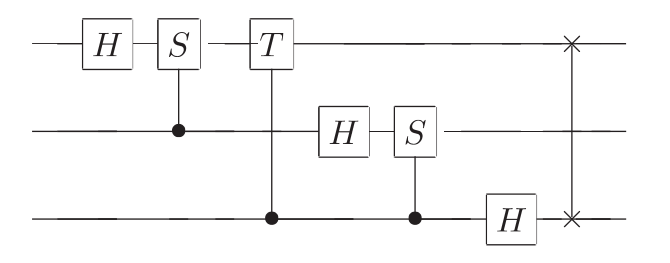
\includegraphics[width=0.75\textwidth]{qft.png}
    \caption{Quantum Fourier Transform Circuit} 
    \label{fig:enter-label}
    \end{center}
\end{figure}

Recall that $S$ and $T$ are the phase and π/8 gates, and $H$ is the Hadamard gate which we mentioned in the introductory sections \cite{niel}.

\begin{itemize}
    \item S gate(phase gate):
    \begin{center}
    \Large
        \[\begin{bmatrix}
            1 & 0 \\
            0 & i
        \end{bmatrix}\]
    \end{center}
    \normalsize
    \item T gate(π/8 gate):
    \begin{center}
    \Large
\[\begin{bmatrix}
    \Large
    1 & 0 \\
    0 & e^{i\pi/4}
    \end{bmatrix}\]    
    \end{center}
\end{itemize}
\normalsize

It's important to note that controlled phase shift gates, which include Controlled-$T$ and Controlled-$S$ gates, are essential in the construction of a \acrshort{qft} circuit.

As with any single \acrshort{qubit} gate one can build a controlled version of the phase shift gate. With respect to the computational basis, the 2-\acrshort{qubit} controlled phase shift gate, shifts the phase with $\varphi$ only if it acts on the state $|11\rangle$\cite{cphase}.

\[
|a,b\rangle \mapsto
\begin{cases}
e^{i\varphi}|a,b\rangle & \text{for } a=b=1 \\
|a,b\rangle & \text{otherwise}
\end{cases}
\]

Controlled Phase gate:
\[
\text{$CR(\phi)$} =
\begin{bmatrix}
    1 & 0 & 0 & 0 \\
    0 & 1 & 0 & 0 \\
    0 & 0 & 1 & 0 \\
    0 & 0 & 0 & e^{i\varphi} \\
\end{bmatrix}
\]

The controlled-$T$ gate is a specific case of the controlled phase gate($CR$), where the phase angle is set to $\phi = \pi/ 4 $.
\[
\text{$CT$} =
\begin{bmatrix}
    1 & 0 & 0 & 0 \\
    0 & 1 & 0 & 0 \\
    0 & 0 & 1 & 0 \\
    0 & 0 & 0 & e^{i\frac{\pi}{4}} \\
\end{bmatrix}
\]

The controlled-S gate is the case where the phase angle is set to $\phi = pi / 2 $ \cite{niel}.

\[
\text{$CS$} =
\begin{bmatrix}
    1 & 0 & 0 & 0 \\
    0 & 1 & 0 & 0 \\
    0 & 0 & 1 & 0 \\
    0 & 0 & 0 & i \\
\end{bmatrix}
\]






As a matrix the quantum Fourier transform in this instance may be written out explicitly, by introducing for simpler notation \Large$\omega= e^{\frac{2\pi i}{8}} = \sqrt{i}$ \normalsize \cite{niel}

\Large

\[
\hat{U}_{QFT}=\frac{1}{\sqrt{8}}
\begin{bmatrix}
1 & 1 & 1 & 1 & 1 & 1 & 1 & 1 \\
1 & \omega & \omega^2 & \omega^3 & \omega^4 & \omega^5 & \omega^6 & \omega^7 \\
1 & \omega^2 & \omega^4 & \omega^6 & 1 & \omega^2 & \omega^4 & \omega^6 \\
1 & \omega^3 & \omega^6 & \omega^1 & \omega^4 & \omega^7 & \omega^2 & \omega^5 \\
1 & \omega^4 & 1 & \omega^4 & 1 & \omega^4 & 1 & \omega^4 \\
1 & \omega^5 & \omega^2 & \omega^7 & \omega^4 & \omega^1 & \omega^6 & \omega^3 \\
1 & \omega^6 & \omega^4 & \omega^2 & 1 & \omega^6 & \omega^4 & \omega^2 \\
1 & \omega^7 & \omega^6 & \omega^5 & \omega^4 & \omega^3 & \omega^2 & \omega^1 \\
\end{bmatrix}
\]
$=$\[
\frac{1}{\sqrt{8}} \begin{bmatrix}
1 & 1 & 1 & 1 & 1 & 1 & 1 & 1 \\
1 & e^{i\frac{\pi}{4}} & e^{i\frac{\pi}{2}} & e^{i\frac{3\pi}{4}} & e^{i\pi} & e^{i\frac{5\pi}{4}} & e^{i\frac{3\pi}{2}} & e^{i\frac{7\pi}{4}} \\
1 & e^{i\frac{\pi}{2}} & e^{i\pi} & e^{i\frac{3\pi}{2}} & 1 & e^{i\frac{\pi}{2}} & e^{i\pi} & e^{i\frac{3\pi}{2}} \\
1 & e^{i\frac{3\pi}{4}} & e^{i\frac{3\pi}{2}} & e^{i\frac{9\pi}{4}} & e^{i\pi} & e^{i\frac{5\pi}{4}} & e^{i\frac{7\pi}{2}} & e^{i\frac{15\pi}{4}} \\
1 & e^{i\pi} & 1 & e^{i\pi} & 1 & e^{i\pi} & 1 & e^{i\pi} \\
1 & e^{i\frac{5\pi}{4}} & e^{i\frac{\pi}{2}} & e^{i\frac{7\pi}{4}} & e^{i\pi} & e^{i\frac{\pi}{4}} & e^{i\frac{\pi}{2}} & e^{i\frac{3\pi}{4}} \\
1 & e^{i\frac{3\pi}{2}} & e^{i\pi} & e^{i\frac{7\pi}{2}} & 1 & e^{i\frac{\pi}{2}} & e^{i\pi} & e^{i\frac{3\pi}{2}} \\
1 & e^{i\frac{7\pi}{4}} & e^{i\frac{3\pi}{2}} & e^{i\frac{15\pi}{4}} & e^{i\pi} & e^{i\frac{3\pi}{4}} & e^{i\frac{7\pi}{2}} & e^{i\frac{15\pi}{4}}
\end{bmatrix}
\]
\normalsize 
\\This representation of the Quantum Fourier Tranform, is going to be very useful to us, when we get to the code implementation.

\chapter{VARIATIONAL QUANTUM CIRCUITS AND ALGORITHMS \label{VQA}}

\section{Variational Quantum Circuits (VQCs)}

Variational quantum circuits, also known as ``parametrized quantum circuits'' or ``adaptable quantum circuits'', are a type of quantum circuit that are used in various applications, such as supervised learning, reinforcement learning, and functional regression. They are designed to harness the potential advantages of quantum computing for solving complex problems. They involve the use of parameterized/variational gates and measurements to encode and manipulate quantum information.

One of the main motivations behind using variational quantum circuits is to take advantage of the expressive power of quantum computing to solve problems that are difficult for classical computers. These circuits are designed to be trainable, meaning that the parameters of the gates can be adjusted to optimize the circuit's performance for a specific task. The optimization process typically involves finding the set of parameters that minimizes a cost or loss function, which is defined based on the specific problem being solvedn\cite{vqc}.

One common approach in variational quantum circuits is to use a hybrid model that combines classical and quantum components. This allows for the use of classical optimization algorithms to update the parameters of the circuit based on feedback from the classical part of the model. This hybrid approach helps to mitigate the noise and errors inherent in current quantum hardware, known as NISQ (Noisy Intermediate-Scale Quantum) devices \cite{vqc2}.

The training process of variational quantum circuits involves updating the parameters of the gates using gradient descent optimization. The gradients of the loss function with respect to the circuit parameters are calculated using the backpropagation method, similar to the calculation in classical neural networks \cite{vqc_arch}. The gradients are then used to update the parameters in the direction that minimizes the loss function.

The performance of variational quantum circuits can be evaluated through numerical simulations and experiments on quantum hardware. Simulations can provide insights into the learning performance and efficiency of the circuits, while experiments on real quantum machines, such as IBMQ systems, can test the applicability and scalability of the circuits in real-world scenarios.

Variational quantum circuits are  an active area of research, and there are ongoing efforts to explore their capabilities and limitations. Theoretical analysis, such as error performance analysis and optimization properties, can provide insights into the representation and generalization powers of variational quantum circuits. Experimental validation on different datasets and problem domains is crucial for understanding the practical usefulness of these circuits.

\section{Variational Quantum Algorithms (VQAs)}

Variational quantum algorithms (\acrshort{vqa}s) are a type of hybrid quantum-classical optimization algorithm that harnesses the capabilities of both classical and quantum computers to solve complex problems \cite{vqa}. \acrshort{vqa}s have emerged as a promising approach in the Noisy Intermediate-Scale Quantum (NISQ) era, where quantum computers are characterized by noise and imperfections.

In \acrshort{vqa}s, the objective function is typically encoded by a VQC, which serves as an ansatz or guess for the ground state of the system. The quantum computer evaluates the objective function by measuring the expectation value of an observable, often the Hamiltonian of the system. The classical optimizer then utilizes this evaluation to update the parameters of the circuit, aiming to minimize the associated cost function \cite{vqa}. Classical optimization methods such as gradient descent can be employed to iteratively adjust the parameters and approach the optimal solution.

It is important to note, that the noise and errors inherent in current quantum hardware present challenges for implementing \acrshort{vqa}s. NISQ devices are prone to errors, and the probability of failed operations is non-negligible. Consequently, \acrshort{vqa}s often rely on shallow circuits or circuits with a significant fraction of failed operations to ensure reliability. However, this limitation can impact the performance of \acrshort{vqa}s and restrict their effectiveness in the presence of noise \cite{limitations}.

One of the various proposed uses of VQCs in combination with an appropriate VQA is the task of quantum compiling \cite{paper}. The aim is to train a VQC to simulate the effect of a quantum operation by training the parameters in the variational gates. For this task one does not try to reach the ground state of a Hamiltonian but rather to minimize the overlap of of the operation produced by the VQC with the target operation. The corresponding VQA consists of devising ansatzes on the VQA structure and designing an efficient construction of the overlap function that plays the role of the cost function. My work falls into this category of VQAs. 

\chapter{QFT VIA A VARIATIONAL QUANTUM CIRCUIT WITH 3 QUBITS}

\label{chap:qft_vqc}

As we mentioned before, \acrshort{qft} is an essential operation in quantum computing. To be realized for $n$ \acrshort{qubit}s this requires 
$\approx n^2$ gates that is an excellent record --taking into account that a general unitary operation
is described by $4^n$ real parameters. On the other hand, this includes controlled-phase gates $R_n$
each of which if to be decomposed into gates from a universal set, requires with the best known
method up today $\approx 20$ gates and an ancillary \acrshort{qubit}. 

In the NIST era the idea of employing fault-tolerant quantum computation has been set aside
since deep-depth circuits are out of discussion. In this work we investigate the question
of realizing the \acrshort{qft} operation with a variational circuit of relatively low depth. Instead of
working with universal set of gates we employ Hamiltonians which can be in principle physically realizable.
 The initial procedure that we follow for a $3$-\acrshort{qubit} is a standard one:
\begin{itemize}
	\item We build an ansantz on the structure of the circuit based on the algebraic properties of \acrshort{qft}.
	\item We define a cost function that measures the distance from the target operation i.e. \acrshort{qft}.
	\item We optimize the parameters in the circuit with a  gradient descent so that the cost is minimized. 
\end{itemize}

  
\section{Building an Ansanz} 

In order to build an ansatz we first take the unitary matrix (in the computational basis), $\hat{U}_{QFT}$,
and we decompose it onto the $64$ generators of $SU(8)$ algebra, i.e. $\hat{g}_{ijk}$,
as 
\begin{equation}
O_{ijk}=Tr\left(\hat{U}_{QFT} \hat{g}_{ijk} \right).
\end{equation}
We find out that only $20$ generators give non-zero overlap $O_{ijk}$.

We commute these $20$ generators and we find out that these together with first, second,.. order commutations form
a closed subgroup of $32$ elements. Then we search for a minimum set of single-\acrshort{qubit} and 2-\acrshort{qubit} operators able to generate the whole
subgroup. We identify $11$ of them ($5$ single \acrshort{qubit} and $6$ two-\acrshort{qubit} Hamiltonians) but possibly this result could be improved.

We build a parametrized circuit that consists of $N$ parametrized gates $\hat{R}_{ijk}$ generated  by these $11$ operators, e.g. $\hat{R}_{ijk}\left(x\right)=\left(I x \hat{g}_{ijk}\right)$. Let us denote by $\hat{U}_c\left(\vec{x}\right)$ the unitary operation describing the parametrized circuit (consisting by a product of $N$ parametrized gates). 
By $\vec{x}=\left\{x_1,\ldots, x_{N}\right\}$ we denote a vector built by the $N$ parameters of the circuit. The aim is to find $\vec{x}$ such that the overlap
 cost function is as low as possible:
\begin{equation}
C\left(\hat{U}_c\left(\vec{x}\right), \hat{U}_{QFT}\right)=1-\frac{1}{64}\left|Tr\left(\hat{U}_c\left(\vec{x}\right)\hat{U}_{QFT}^{\dagger} \right)\right|^2. \label{C}
\end{equation}
The cost function $C$ is constructed such a way \cite{paper} so that this takes value in the interval $\left[0,1\right]$
with $C=0$ corresponding to the case where $\hat{U}_c\left(\vec{x}\right)= \hat{U}_{QFT}$ up to a global phase.
By augmenting $N$ naturally one expects better results since this way more `volume' in the space of unitary matrices can be covered by the VQC.  I also note here that the structure of circuit is not crucial provided that some simple logical rules are followed such that  there is full connectivity of all qubits and that there is no successive single qubit gates on the same qubit.



\section{Gradient Descent Optimizer}

Before we move on to the code implementation, it is important to give some information about the optimization method I used for this project. 

Gradient descent is an iterative optimization algorithm used to find the local minimum of a differentiable function. It is particularly useful in machine learning for minimizing the cost or loss function. The basic idea behind gradient descent is to take repeated steps in the opposite direction of the gradient of the function at the current point, because this is the direction of steepest descent. By iteratively updating the parameters in the direction of the negative gradient, the algorithm gradually converges towards a minimum point \cite{gradient}.

To understand gradient descent, let's consider an analogy. Imagine a person who is stuck in the mountains and is trying to find the lowest point (i.e., the global minimum). Due to heavy fog, the person cannot see the path down the mountain. Instead, they must rely on local information to find the minimum. In this scenario, the person can use the method of gradient descent. They look at the steepness of the hill at their current position and proceed in the direction with the steepest descent (i.e., downhill). If they were trying to find the top of the mountain (i.e., the maximum), they would proceed in the direction of steepest ascent (i.e., uphill).

In the context of machine learning, gradient descent is used to update the parameters of a model in order to minimize the cost or loss function. The parameters refer to the coefficients in linear regression or the weights in neural networks \cite{gradient}. The goal is to find the parameter values that minimize the cost function, which represents the discrepancy between the predicted values and the actual values in the training data \cite{gd}.

There are different variations of gradient descent, including batch gradient descent, mini-batch gradient descent and stochastic gradient descent, which is also tested in this project.

In stochastic gradient descent, the algorithm calculates the gradient of the cost function with respect to a single training example in each iteration and updates the parameters based on this gradient. This method is computationally efficient but can have high variance in the parameter updates, leading to slower convergence. However, it can escape local minima and find better solutions \cite{gradient}.

The choice of which variation of gradient descent to use depends on the specific problem and the available computational resources. For example, batch gradient descent is typically used when the dataset can fit into memory and computational efficiency is not a major concern. On the other hand, stochastic gradient descent and mini-batch gradient descent are often preferred for large datasets or when computational efficiency is important \cite{gd}.

\chapter{RESULTS \label{results}}

In order to reach to conclusions, I run multiple tests, for different number of parameters, $N$, using a different combination of hyperparameters for the gradient descent optimizer. I start from a random initial point \textbf{X INITIAL}$=\vec{x}_{init}$ in the parameter space and the aim is to reach by gradient descent an optimum set of parameters \textbf{X FINAL}$=\vec{x}_{fin}$ so that the  overlap cost function in Eq. (\ref{C}) is minimized. I repeat the procedure for more initial points and I pick the result providing the lowest cost. 

\section{18 parameters}
\begin{enumerate}[label=\textbf{\Alph*.}]
\item \textbf{ }
\begin{figure}[H]
\begin{center}
    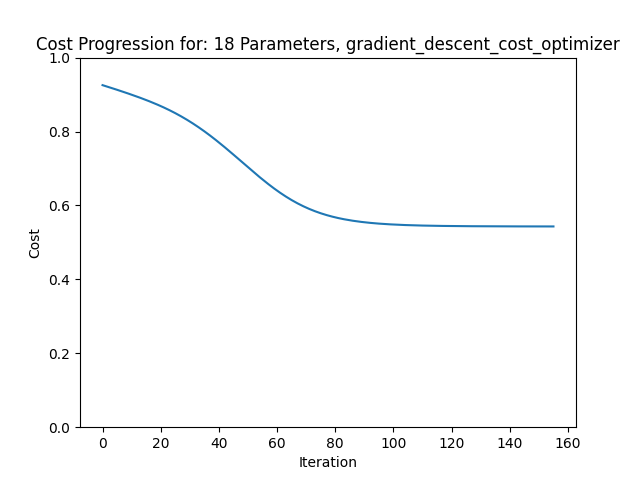
\includegraphics[width=0.9\textwidth]{plots/18.png}
    \caption{Cost progression plot, with 18 trainable parameters, using Gradient Descent optimizer(A)} 
    \label{fig:enter-label}
    \end{center}
\end{figure}

It is obvious, that in this particular snapshot, the final cost is not the optimal result.

Here are the initial and the final parameter values, as well as the initial and final costs. \\

\textbf{X INITIAL} is:
 tensor([1.7658, 3.4312, 4.1421, 5.3068, 0.1327, 5.7904, 4.1582, 1.2668, 5.6374,
        6.0970, 2.9710, 1.6479, 0.6261, 2.5107, 3.8973, 3.1691, 0.1296, 4.8192])

\textbf{initial cost}: tensor(0.9279)

\textbf{X FINAL} is:
 tensor([1.4667, 4.2022, 4.2278, 5.2510, 0.1786, 6.2554, 3.9019, 1.3128, 5.7231,
        6.0693, 3.4226, 1.6939, 0.3527, 2.5964, 4.2336, 2.5559, 0.2154, 4.8651]),

\textbf{final cost}: tensor(0.5432)

learning rate =  0.05\\ 
delta =  0.005 \\
epsilon =  1e-08 \\
threshold =  1e-05 \\
step size =  0.1 \\

More information about how the code is implemented, are in the appendix.

Some other implementations with 18 parameters gave similar results.

\item \textbf{ }
\begin{figure}[H]
\begin{center}
    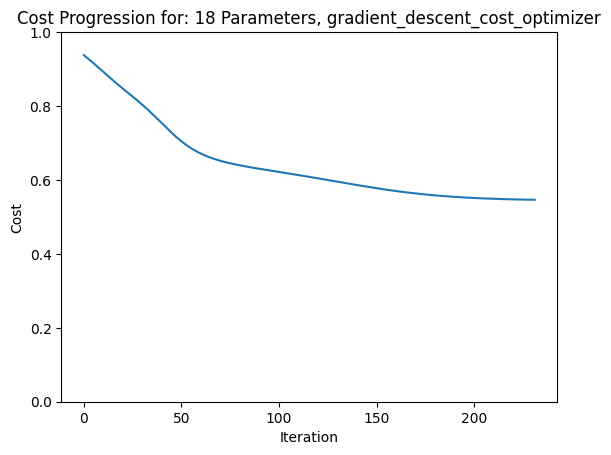
\includegraphics[width=0.9\textwidth]{18.png}
    \caption{Cost progression plot, with 18 trainable parameters, using Gradient Descent optimizer(B)} 
    \label{fig:enter-label}
    \end{center}
\end{figure}

\textbf{X INITIAL} is: tensor([4.8274, 1.5107, 1.5987, 3.6443, 5.9472, 2.8795, 0.4899, 4.3089, 1.4795,
        4.2034, 3.8087, 0.3544, 0.4266, 2.9152, 0.2256, 1.8776, 4.5090, 0.9238])
        
\textbf{initial cost}: = tensor(0.9416)

\textbf{X FINAL} is: tensor([4.6312, 1.1150, 1.3784, 3.7199, 5.8616, 3.2902, 0.7585, 4.2233, 1.2592,
        4.4295, 3.5401, 0.2688, 0.3703, 2.6949, 1.0287, 2.5523, 4.2887, 0.8382])
        
\textbf{final cost}: tensor(0.5464)

learning rate =  0.05 \\
delta =  0.005 \\
epsilon =  1e-08 \\
threshold =  0.001 \\
step size =  0.1 \\

\item \textbf{ }
In this last case, I decided to run the program with different parameters for the gradient descent. Instead of the previous "epsilon" value(1e-08) I choose to increase it to 1e-06.
\begin{figure}[H]
\begin{center}
    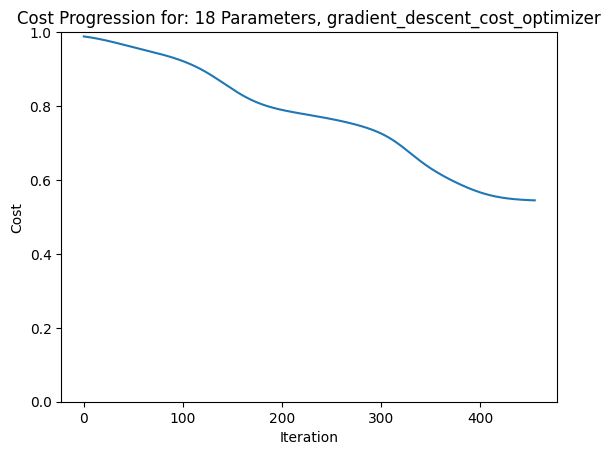
\includegraphics[width=0.9\textwidth]{epsilon06/18.png}
    \caption{Cost progression plot, with 18 trainable parameters, using Gradient Descent optimizer(C)} 
    \label{fig:enter-label}
    \end{center}
\end{figure}

\textbf{X INITIAL} is:
 tensor([1.4468, 6.1483, 5.0250, 2.7024, 1.6291, 0.2811, 4.5268, 0.7270, 2.9660,
        4.9462, 4.7656, 0.4019, 0.4443, 6.2669, 3.6787, 3.4641, 5.6090, 2.2776])
        
\textbf{initial cost}: = tensor(0.9887)

\textbf{X FINAL is}:
tensor([ 1.4848,  5.7350,  4.8197,  2.8080,  1.5974,  0.2750,  3.9014,  0.6953,
         2.7608,  4.7029,  4.7299,  0.3702, -0.3118,  6.0617,  2.6975,  2.5539,
         5.4037,  2.2459])

\textbf{final cost}: tensor(0.5449)\\

learning rate =  0.05 \\
delta =  0.005 \\
epsilon =  1e-06 \\
threshold =  0.0001\\
step size =  0.1 \\

\end{enumerate}

After multiple executions with 18 parameters, I realized that the final cost would not get lower than 0.5. As a result, more parameters are needed to train this circuit and minimize the cost. 

\section{20 parameters}

\begin{figure}[H]
\begin{center}
    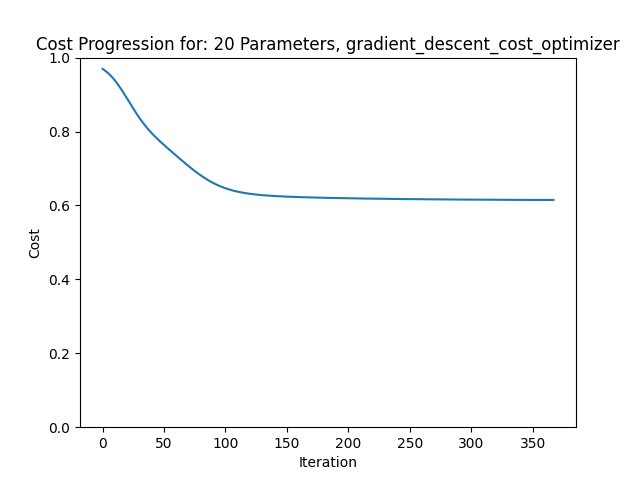
\includegraphics[width=0.9\textwidth]{20.png}
    \caption{Cost progression plot, with 20 trainable parameters, using Gradient Descent optimizer} 
    \label{fig:enter-label}
    \end{center}
\end{figure}

\textbf{X INITIAL} is: tensor([3.1948, 5.3759, 4.9216, 0.6639, 0.7274, 1.3457, 4.1867, 3.4602, 3.4542,
        3.5626, 2.9046, 5.0324, 1.6932, 1.5336, 2.8378, 5.3266, 2.7702, 1.1606,
        1.8269, 0.3608])

\textbf{initial cost}: tensor(0.9716)

\textbf{X FINAL} is: tensor([2.8576, 5.6991, 5.1387, 0.9144, 0.7338, 1.1805, 3.8612, 3.4666, 3.6713, 3.6662, 3.3033, 5.0389, 2.3572, 1.7507, 3.0914, 4.9087, 2.9874, 1.1671, 1.9527, 1.1274])

\textbf{final cost}: tensor(0.6147)

learning rate =  0.05 \\
delta =  0.005 \\
epsilon =  1e-08 \\
threshold =  0.0001\\
step size =  0.1 \\

After multiple executions, I concluded that I need to increase the parameters a little more, since 20 parameters are not enough.

\section{22 parameters}

\begin{enumerate}[label=\textbf{\Alph*.}]
    \item \textbf{ }

    \begin{figure}[H]
        \centering
        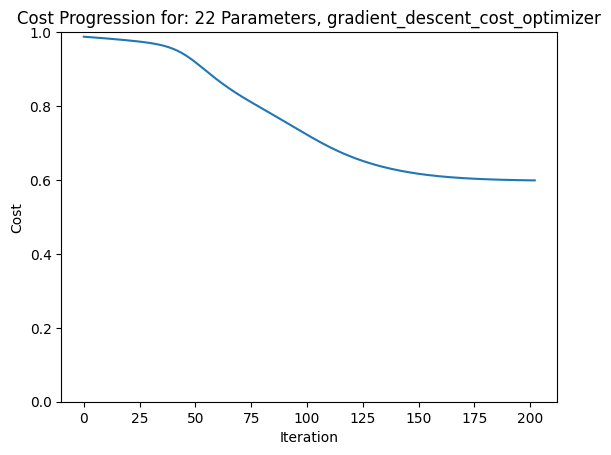
\includegraphics[width=0.9\textwidth]{22.png}
        \caption{Cost progression plot, with 22 trainable parameters, using Gradient Descent optimizer(A)} 
        \label{fig:fig1}
    \end{figure}

    \textbf{X INITIAL} is:
    tensor([5.5316, 4.8904, 5.3289, 0.0076, 3.5166, 1.9878, 4.1190, 3.4012, 2.7321,
            3.2201, 5.3298, 1.9683, 1.6896, 3.9811, 0.0533, 3.2435, 1.0930, 5.2226,
            2.2948, 0.1961, 1.6848, 4.0577])
            
    \textbf{initial cost}: tensor(0.9880)
    
    \textbf{X FINAL} is:
    
    tensor([ 5.8946,  5.8026,  5.4321,  0.3726,  3.4180,  2.2436,  3.9729,  3.3026,
             2.8353,  2.7521,  5.6147,  1.8697,  2.3123,  4.0844, -0.0451,  3.3367,
             1.1963,  5.1240,  2.1425,  0.0551,  1.4876,  4.3096])
    
    \textbf{final cost}: tensor(0.5989)
    
    learning rate =  0.05 \\
    delta =  0.005 \\
    epsilon =  1e-08 \\
    threshold =  0.0001\\
    step size =  0.1 \\
    
    \item \textbf{ }

    Instead of the previous "epsilon" value (1e-08), I chose to increase it to 1e-06.

    \begin{figure}[H]
        \centering
        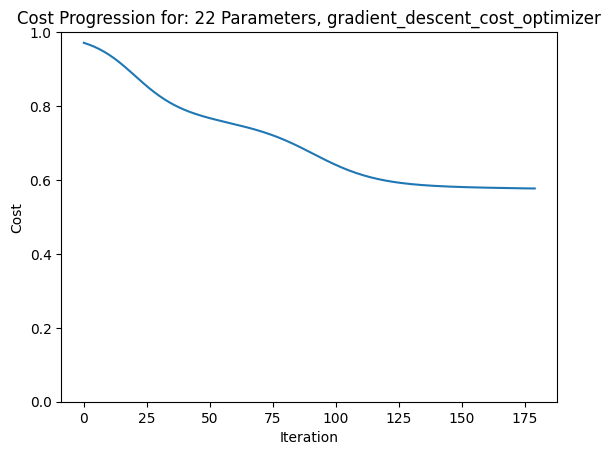
\includegraphics[width=0.9\textwidth]{epsilon06/22.png}
        \caption{Cost progression plot, with 22 trainable parameters, using Gradient Descent optimizer(B)} 
        \label{fig:fig2}
    \end{figure}

    \textbf{X INITIAL} is:
    tensor([3.4730, 2.6421, 5.1826, 1.7041, 5.8734, 3.2929, 1.7257, 2.0646, 2.5464,
           6.2450, 0.6135, 3.7199, 2.8965, 3.6478, 2.8020, 1.7141, 0.3224, 5.4836,
           1.1351, 5.5521, 1.8220, 3.1569])
           
    \textbf{initial cost}: tensor(0.9731)

    \textbf{X FINAL} is:
    tensor([3.0353, 2.8943, 5.0558, 1.5389, 5.8523, 3.0472, 2.2930, 2.0435, 2.4196,
           6.0623, 0.5559, 3.6988, 3.1135, 3.5210, 3.0138, 0.9943, 0.1956, 5.4625,
           1.4578, 5.3369, 1.7798, 3.2443])

    \textbf{final cost}: tensor(0.5770)

    learning rate =  0.05 \\
    delta =  0.005 \\
    epsilon =  1e-06 \\
    threshold =  0.0001\\ 
    step size =  0.1 \\

\end{enumerate}

\section{26 parameters}

\begin{enumerate}[label=\textbf{\Alph*.}]
    \item \textbf{ }
    
    \begin{figure}[H]
        \centering
        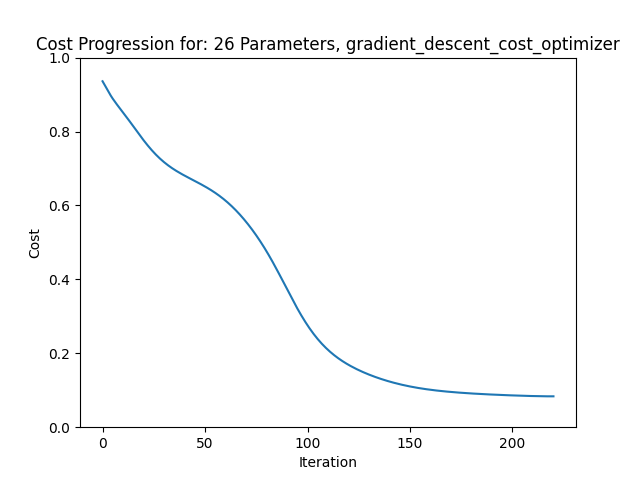
\includegraphics[width=0.9\textwidth]{26.png}
        \caption{Cost progression plot, with 26 trainable parameters, using Gradient Descent optimizer(A)} 
        \label{fig:fig1}
    \end{figure}
    
    \textbf{X INITIAL} is:
    tensor([3.2022, 5.6416, 4.8515, 3.3115, 3.6187, 5.0852, 2.9730, 5.0537, 1.5072,
            4.7531, 0.5125, 5.5763, 5.8622, 1.1606, 0.6496, 2.2168, 3.9991, 5.3104,
            4.2755, 3.8328, 1.0954, 1.9451, 4.8207, 4.8218, 4.6000, 1.4309])
            
    \textbf{initial cost}: tensor(0.9451)
    
    \textbf{X FINAL} is: 
    tensor([2.3827, 5.2529, 4.6696, 3.5108, 3.6095, 5.0535, 3.9956, 5.2220, 1.1325,
            4.1914, 0.7261, 5.7447, 5.8750, 0.7859, 0.9014, 2.5525, 3.6244, 5.4788,
            3.8632, 4.2661, 0.9771, 2.2849, 5.1514, 4.4313, 4.2616, 1.4216])
    
    \textbf{final cost}: tensor(0.0836)
    
    learning rate =  0.05 \\
    delta =  0.005 \\
    epsilon =  1e-08 \\
    threshold =  0.0001\\ 
    step size =  0.1 \\
    
    \item \textbf{ }
    
    \begin{figure}[H]
        \centering
        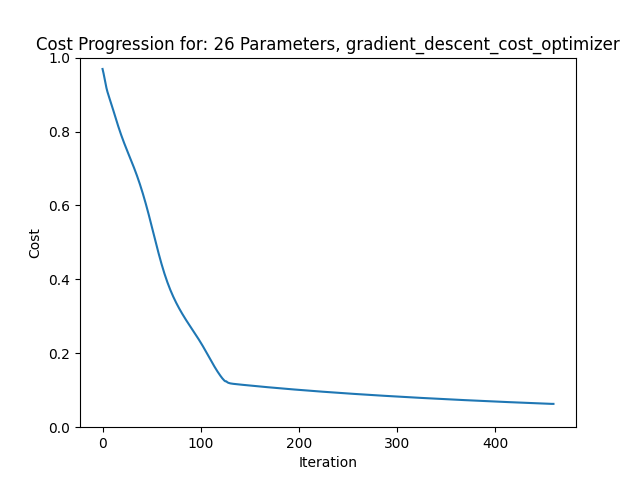
\includegraphics[width=0.9\textwidth]{26_b.png}
        \caption{Cost progression plot, with 26 trainable parameters(b), using Gradient Descent optimizer(B)} 
        \label{fig:fig2}
    \end{figure}
    
    \textbf{X INITIAL} is:
    tensor([2.8648, 5.4188, 0.7875, 4.8503, 4.0227, 1.7765, 1.3553, 0.6937, 5.7583,
            0.8078, 4.9534, 1.9077, 6.2795, 0.9409, 3.3676, 0.6460, 3.6312, 4.4370,
            5.8479, 5.9351, 5.4692, 2.7993, 3.0437, 3.2066, 5.3126, 2.4545])
            
    \textbf{initial cost}: tensor(0.9781)
    
    \textbf{X FINAL} is:
    
    tensor([3.3034, 5.5917, 0.8085, 4.6238, 4.3980, 1.5872, 0.9654, 0.7109, 5.4160,
            1.0719, 4.8915, 1.9250, 5.3130, 0.5986, 4.1386, 0.9808, 3.2889, 4.4543,
            5.9470, 5.9129, 5.4806, 2.7109, 3.6705, 2.8900, 5.2372, 2.8299])
    
    \textbf{final cost}: tensor(0.0631)
    
    learning rate =  0.05 \\
    delta =  0.005 \\
    epsilon =  1e-08 \\
    threshold =  0.0001\\ 
    step size =  0.1 \\
    
    \item{ }
    
    Instead of the previous "epsilon" value(1e-08), I choose to increase it to 1e-06.
    
    \begin{figure}[H]
        \centering
        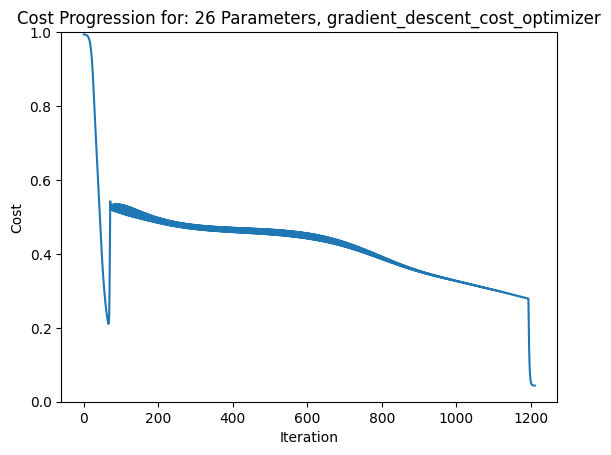
\includegraphics[width=0.9\textwidth]{epsilon06/26.png}
        \caption{Cost progression plot, with 26 trainable parameters(c), using Gradient Descent optimizer(C)} 
        \label{fig:fig3}
    \end{figure}
    
    \textbf{X INITIAL} is:
    tensor([2.8710, 4.7578, 3.3982, 1.5568, 5.3054, 0.7483, 4.1578, 3.5420, 2.4154,
            4.7246, 5.3815, 0.3457, 2.7512, 2.6583, 5.3696, 4.0464, 1.9786, 3.5664,
            5.2470, 1.9843, 6.2567, 0.6134, 1.5815, 5.8635, 5.9813, 2.5164])
            
    \textbf{initial cost}: tensor(0.9940)
    
    \textbf{X FINAL} is:
    tensor([ 1.3361,  5.7477,  3.3366,  2.1055,  5.4184, -0.1233,  4.2182,  3.1592,
             2.1595,  5.3936,  5.6810, -0.0371,  1.3140,  2.4024,  5.8358,  4.1234,
             1.7227,  3.1837,  5.0808,  2.3511,  6.2768,  0.7038,  1.5699,  6.0155,
             5.3044,  2.6294])
             
    \textbf{final cost}: tensor(0.0437)

    learning rate =  0.05 \\
    delta =  0.005 \\
    epsilon =  1e-06 \\
    threshold =  0.0001\\ 
    step size =  0.1 \\
    
    After testing the circuit for 18, 20, and 22 parameters, on 26 parameters, the result is optimal. The cost is minimized and is equal to 0.0437.
    
\end{enumerate}

\section{28 parameters}

\begin{enumerate}[label=\textbf{\Alph*.}]
    \item \textbf{  }
    
    \begin{figure}[H]
        \centering
        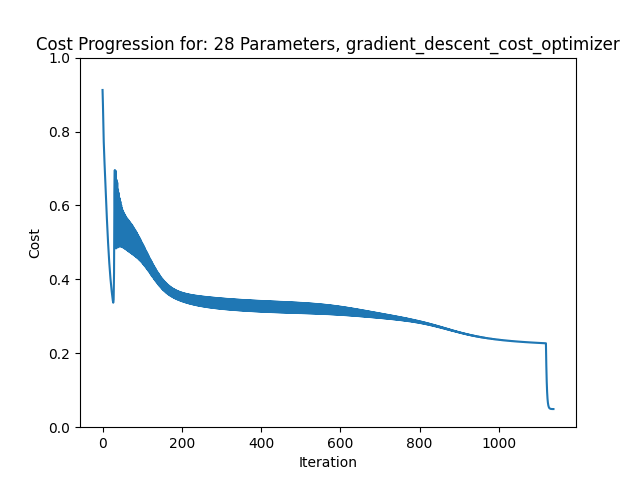
\includegraphics[width=0.9\textwidth]{28.png}
        \caption{Cost progression plot, with 28 trainable parameters, using Gradient Descent optimizer(A)} 
        \label{fig:fig1}
    \end{figure}
    
    \textbf{X INITIAL} is:
    tensor([3.6285, 0.5717, 1.3463, 0.2393, 3.4633, 1.5723, 6.1080, 5.0117, 4.5497,
            1.1938, 5.7585, 1.8747, 2.4548, 3.4901, 4.9434, 3.3576, 0.2792, 4.1673,
            3.8621, 2.6452, 4.2201, 5.2078, 4.3327, 5.5728, 5.9729, 0.1138, 2.8426,
            4.2832])
            
    \textbf{initial cost}: tensor(0.9368)
    
    \textbf{X FINAL} is:
    tensor([ 2.7217,  0.4280,  0.1943,  0.3745,  3.3493,  1.4766,  6.7955,  5.2375,
             4.6558,  0.7024,  5.9003,  2.1004,  2.4367,  3.5962,  3.9115,  3.3380,
             0.3853,  4.3931,  3.5211,  2.5860,  3.9345,  5.3438,  3.9282,  5.4054,
             5.5653, -0.0083,  3.1441,  4.0902])
    
    \textbf{final cost}: tensor(0.0491)
    
    learning rate =  0.05 \\
    delta =  0.005 \\
    epsilon =  1e-08 \\
    threshold =  0.0001\\ 
    step size =  0.1
    
    \item \textbf{  }
    
    \begin{figure}[H]
        \centering
        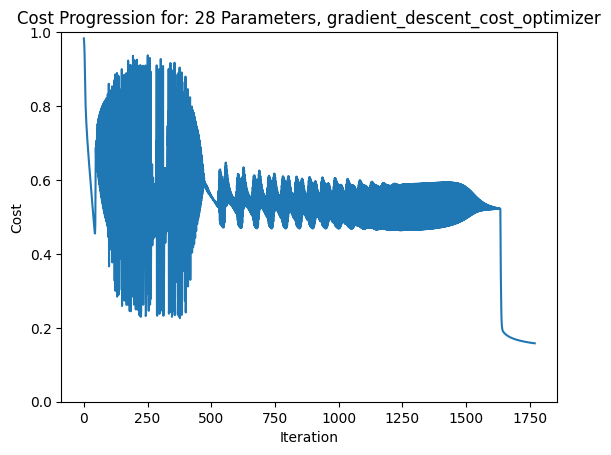
\includegraphics[width=0.9\textwidth]{plots/28s.png}
        \caption{Cost progression plot, with 28 trainable parameters, using Gradient Descent optimizer(B)} 
        \label{fig:fig2}
    \end{figure}
    
    \textbf{X INITIAL}  is:
    tensor([4.5330, 1.2127, 5.8686, 3.9970, 6.0627, 3.8046, 3.1711, 3.8535, 0.4302,
            4.0036, 2.4540, 5.2031, 2.1072, 1.0062, 4.4468, 0.7581, 1.1217, 2.6496,
            4.4254, 2.6519, 1.4644, 3.2951, 4.1166, 5.0768, 0.5094, 2.3641, 4.8506,
            3.9727])
            
    \textbf{initial cost}: tensor(0.9884)
    
    \textbf{X FINAL} is:
    tensor([4.9584, 1.3110, 6.6644, 3.9844, 6.1405, 4.0523, 3.8551, 2.9820, 0.6069,
            4.5222, 1.5677, 4.3316, 2.9369, 1.1830, 4.8590, 0.1916, 1.2984, 1.7781,
            4.4359, 2.7650, 1.8271, 3.5744, 4.3506, 5.0568, 0.6657, 1.9018, 4.3499,
            3.3173])
    
    \textbf{final cost}: tensor(0.1581)
    
    learning rate =  0.05 \\
    delta =  0.005 \\
    epsilon =  1e-08 \\
    threshold =  0.0001\\ 
    step size =  0.1 \\
    
    \item{ }
    
    Lets test it with "epsilon" = 1e-06.
    
    \begin{figure}[H]
        \centering
        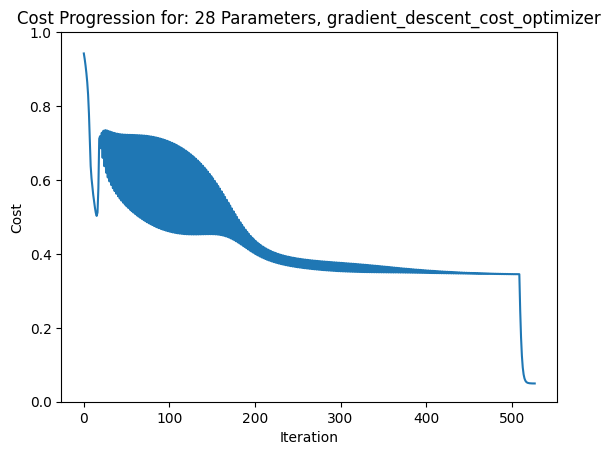
\includegraphics[width=0.9\textwidth]{epsilon06/28.png}
        \caption{Cost progression plot, with 28 trainable parameters, using Gradient Descent optimizer(C)} 
        \label{fig:fig3}
    \end{figure}
    
    \textbf{X INITIAL}  is:
    tensor([2.0370, 1.5601, 2.9670, 5.9147, 1.7438, 4.8593, 0.8470, 0.8450, 5.3775,
            1.0312, 4.9395, 2.6428, 1.3595, 4.7149, 1.6253, 2.5752, 3.9885, 3.9920,
            5.5750, 2.4976, 4.4143, 0.8474, 6.2534, 5.4128, 3.5603, 3.2367, 2.3206,
            1.7052])
            
    \textbf{initial cost}: tensor(0.9539)
    
    \textbf{X FINAL} is:
    tensor([2.4495, 1.5559, 3.4123, 5.9498, 2.6323, 3.9259, 1.4310, 0.4180, 5.1273,
            0.5496, 5.4894, 2.2158, 1.0248, 4.4646, 1.7050, 2.5476, 3.7383, 3.5650,
            5.6853, 2.5584, 4.7759, 0.8392, 6.1957, 5.5991, 4.2603, 2.7112, 2.9145,
            1.8037])
    
    \textbf{final cost}: tensor(0.0494)
    
    learning rate =  0.05 \\
    delta =  0.005 \\
    epsilon =  1e-06 \\
    threshold =  0.0001 \\
    step size =  0.1 \\
    
\end{enumerate}

\section{36 parameters}

\begin{enumerate}[label=\textbf{\Alph*.}]
    \item \textbf{  }
    
    \begin{figure}[H]
        \centering
        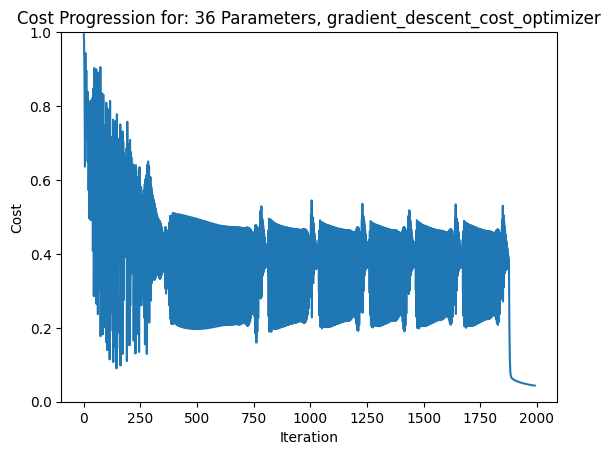
\includegraphics[width=0.9\textwidth]{36_08.png}
        \caption{Cost progression plot, with 36 trainable parameters, using Gradient Descent optimizer (A)} 
        \label{fig:fig4}
    \end{figure}
    
    \textbf{X INITIAL}  is:
    tensor([4.8362, 3.6321, 3.6455, 5.0998, 3.9771, 3.4398, 2.6750, 1.2670, 4.5698,
            0.5346, 4.9464, 5.9116, 5.6344, 2.2204, 1.3853, 2.7208, 4.4199, 2.4230,
            0.8827, 5.6453, 5.6098, 6.0475, 5.0129, 5.9373, 3.6265, 1.8172, 0.2852,
            3.4911, 4.7342, 2.6652, 0.2896, 3.0127, 0.6324, 3.9121, 5.5221, 2.0697])
            
    \textbf{initial cost}: tensor(0.9984)
    
    \textbf{X FINAL} is:
    tensor([5.0624, 3.4483, 3.9738, 4.6945, 4.5981, 2.7576, 2.7066, 1.1965, 4.7613,
            0.6210, 4.8822, 5.8412, 5.8972, 2.4119, 1.2588, 2.7085, 4.6114, 2.3525,
            1.0755, 5.5077, 5.8030, 5.8436, 4.6022, 5.8765, 3.9150, 1.7130, 0.5636,
            3.0456, 4.8265, 2.0078, 0.1334, 2.5234, 0.5314, 3.8751, 4.9492, 2.6907])
    
    \textbf{final cost}: tensor(0.0437)
    
    learning rate =  0.05 \\
    delta =  0.005 \\
    epsilon =  1e-08 \\
    threshold =  0.0001\\ 
    step size =  0.1 \\
    
    \item { }
    
    Again changing epsilon to 1e-06:
    
    \begin{figure}[H]
        \centering
        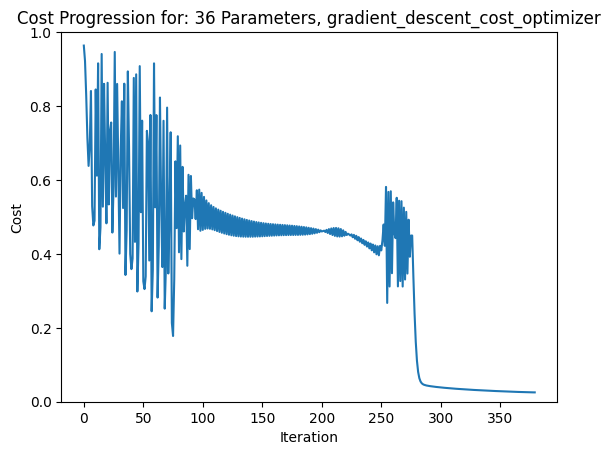
\includegraphics[width=0.9\textwidth]{epsilon06/36b.png}
        \caption{Cost progression plot, with 36 trainable parameters, using Gradient Descent optimizer (B)} 
        \label{fig:fig5}
    \end{figure}
    
    \textbf{X INITIAL}  is:
    tensor([5.9952, 5.5263, 0.6751, 6.0429, 2.1922, 0.3648, 5.7690, 6.0980, 3.3402,
            1.8612, 2.8357, 2.1689, 5.5096, 4.7071, 5.0906, 4.2524, 2.3970, 0.8527,
            3.8382, 4.1531, 3.7767, 1.5861, 5.9046, 4.4120, 0.5971, 2.0312, 1.8445,
            5.6879, 4.9407, 4.7796, 5.3012, 4.8495, 5.8104, 0.8958, 3.2829, 6.1114])
            
    \textbf{initial cost}:  tensor(0.9840)
    
    \textbf{X FINAL} is:
    tensor([5.9893, 5.3949, 0.6761, 5.9251, 2.5392, 0.2661, 5.6742, 6.2167, 3.2759,
            1.5737, 2.7046, 2.2876, 5.5921, 4.6428, 4.4534, 4.2063, 2.3327, 0.9713,
            3.6880, 4.0220, 3.6738, 1.6063, 5.5940, 4.3295, 0.9447, 1.7410, 2.2376,
            5.3814, 4.9522, 4.8468, 5.0590, 4.5405, 6.0542, 0.7577, 3.0983, 6.4584])
    
    \textbf{final cost}:  tensor(0.0253)
    
    learning rate =  0.05 \\
    delta =  0.005 \\
    epsilon =  1e-06 \\
    threshold =  0.0001 \\
    step size =  0.1 \\
    
\end{enumerate}

\section{Execution time comparison}

\textbf{System specs} \\
CPU: i7 9750h (6 cores - 12threads)\\
RAM: 16GB DDR4\\

\begin{table}[htbp]
  \centering
  \caption{Optimization Results for different number, $N$, of parameters and different Epsilon Values}
  \label{tab:results}
  \begin{tabular}{cccccc}
    \toprule
    \textbf{\# of parameters} & \textbf{Epsilon} & \textbf{Iterations} & \textbf{Final Cost} & \textbf{Execution time} \\
    & & & \\
    \midrule
    18 & 1e-08   & 231 & 0.5464 & 12998.27 (3h 36m 38s) \\
       & 1e-06   & 455 & 0.5449 & 5266.01 (1h 27m 46s) \\
    \midrule
    22 & 1e-08   & 202 & 0.5989 & 3767.74 (1h 2m 47s) \\
       & 1e-06   & 179 & 0.5770 & 3209.74 (53m 29s) \\
    \midrule
    26 & 1e-08   & 220  & 0.0836 & 26892.91 (7h 28m 12s) \\
       & 1e-06   & 1211 & 0.0437 & 27805.79 (7h 43m 25s) \\
    \midrule
    28 & 1e-08   & 1770 & 0.1581 & 45584.77 (12h 39m 45s) \\
       & 1e-06   & 527  & 0.0494 & 12425.25 (3h 27m 5s) \\
    \midrule
    36 & 1e-08   & 1991 & 0.0437 & 84463.23 (23h 27m 43s) \\
       & 1e-06   & 379  & 0.0253 & 16445.67 (4h 34m 6s) \\
    \bottomrule
  \end{tabular}
\end{table}


\chapter{CONCLUSIONS AND FUTURE WORK}

\section{Conclusions}

The results showed that increasing the number of trainable parameters in the quantum circuit generally improved the result of optimization process. Starting from 18 parameters, the cost decreased as more parameters were added, indicating that a larger parameter space allows for better optimization and lower cost values. Significant results, were achieved for the first time, on 26 parameters. Also, the initial parameters seemed to have an important impact on the optimization process. Different initializations resulted in different convergence rates and final cost values, even though for more than 26 parameters, the cost was always successfully optimized. This is an interesting point since it implies that even though the number of local minima is increasing with the number of parameters, these minima are of equal depth/value. This effect has not been mentioned in other optimization tasks attacked with VQCs where usually barren plateaus appear.

The findings also reveal another interesting aspect of the optimization process: When dealing with a considerable number of parameters(in this case $N=$28 and 36), and as the number of parameters increases, adjusting the epsilon value from 1e-08 to 1e-06 had a notable impact on both execution time and the number of iterations required for convergence. 
While this change slightly affected the final cost, the benefits in terms of resource savings were substantial, outweighing the marginal degradation in the cost function. Specifically, adopting a greater epsilon value accelerated the optimization process significantly. By increasing epsilon, the optimizer could take more substantial steps during each iteration, expediting the convergence towards an optimal solution. As a result, fewer iterations were needed to reach a satisfactory cost value, leading to a reduction in the overall execution time of the optimization algorithm.

%?????????Although the final cost might have been slightly compromised???? compared to the case with a larger epsilon value, the importance of conserving computational resources cannot be overlooked. The gains in execution time are of great significance, particularly in scenarios where quantum circuits grow in complexity and size, as optimization times tend to scale accordingly. Additionally, the difference in the final cost resulting from the epsilon adjustment was not substantial, indicating that the solution obtained was still highly effective for practical purposes.

To summarize,  the epsilon value played a crucial role not only in influencing the final cost but also in significantly impacting the optimization process's speed and resource efficiency. Fine-tuning this hyperparameter allowed for a more balanced trade-off between solution quality and computational requirements, making the overall optimization procedure more viable and scalable for real-world quantum computing applications. 

The cost progression plots provided a useful way to visualize the optimization process, showing how the cost evolved over iterations, and whether the algorithm was converging or getting stuck in local minima. For most configurations, the cost progression plots showed that the optimization process was converging towards a minimum cost value, indicating that the quantum circuit was being trained successfully.

The experiments suggest that to efficiently train this specific quantum circuit, 26 parameters were found to be sufficient. Adding more parameters beyond this threshold did not lead to significant improvements in the final cost. Even though the best result was achieved with 36 trainable parameters, with the lowest cost value of 0.0253 using Gradient Descent optimizer (B) and an epsilon value of 1e-06, the difference between the cost produced by 26 parameters(0.0437), or 28 parameters(0.094) is not significant. A generic random unitary would require a VQC with at least $64$ parameters to reach such a value of cost function and thus I can safely conclude that the algebraic ansatz which I have used has proven advantageous reducing the number of parameters and consequently the depth of quantum circuit in half. Notably, I performed an experiment with random generators outside from the set provided by the ansatz and the cost reached was larger by an order of magnitude (for $N=26$ parameters).

In conclusion, the experiments showed that the optimization process of a quantum circuit heavily relies on the number of parameters and hyperparameter tuning. It is essential to find the right balance between complexity and computational efficiency to achieve an optimal solution for the specific quantum circuit under consideration.

As a future work I would like to proceed with 4 and 5 qubit VQC and investigate how my observations keep up in these cases. Even though my VQC consists of a circuit of larger  depth  than the initial compilation of QFT (see Figure \ref{fig:enter-label} ), one should take into account that the proposed VQC in this work can compile other operations as well with the same architecture and thus is more generic and powerful. In conclusion  my results give some promise that this important operation in quantum computing could be realized  by VQC obeying certain algebraic structure. In addition the training of such VQC is executable on a classical computer if the optimization methods and parameters withing are thoughtfully selected.

\chapter{APPENDIX}
\section{Python implementation}

This project is implemented in python, using mostly the \textbf{PyTorch} library. 

Gradient descent, as well as stochastic gradient descent are implemented from scratch following the mathematical formula, since the optimizers included in \textbf{PyTorch} library, were not suitable for this type of model. The final circuit is a $8\times8$ matrix, that is imposible to be optimized by using simply the \textbf{torch.optim} package. The full code, implemented in python, is stated below in \textbf{Google Collab} notebook form. The stochastic gradient descent is implemented in the code bellow, but it is not used since it turned out to be ineffective for the needs of this project. \\ 

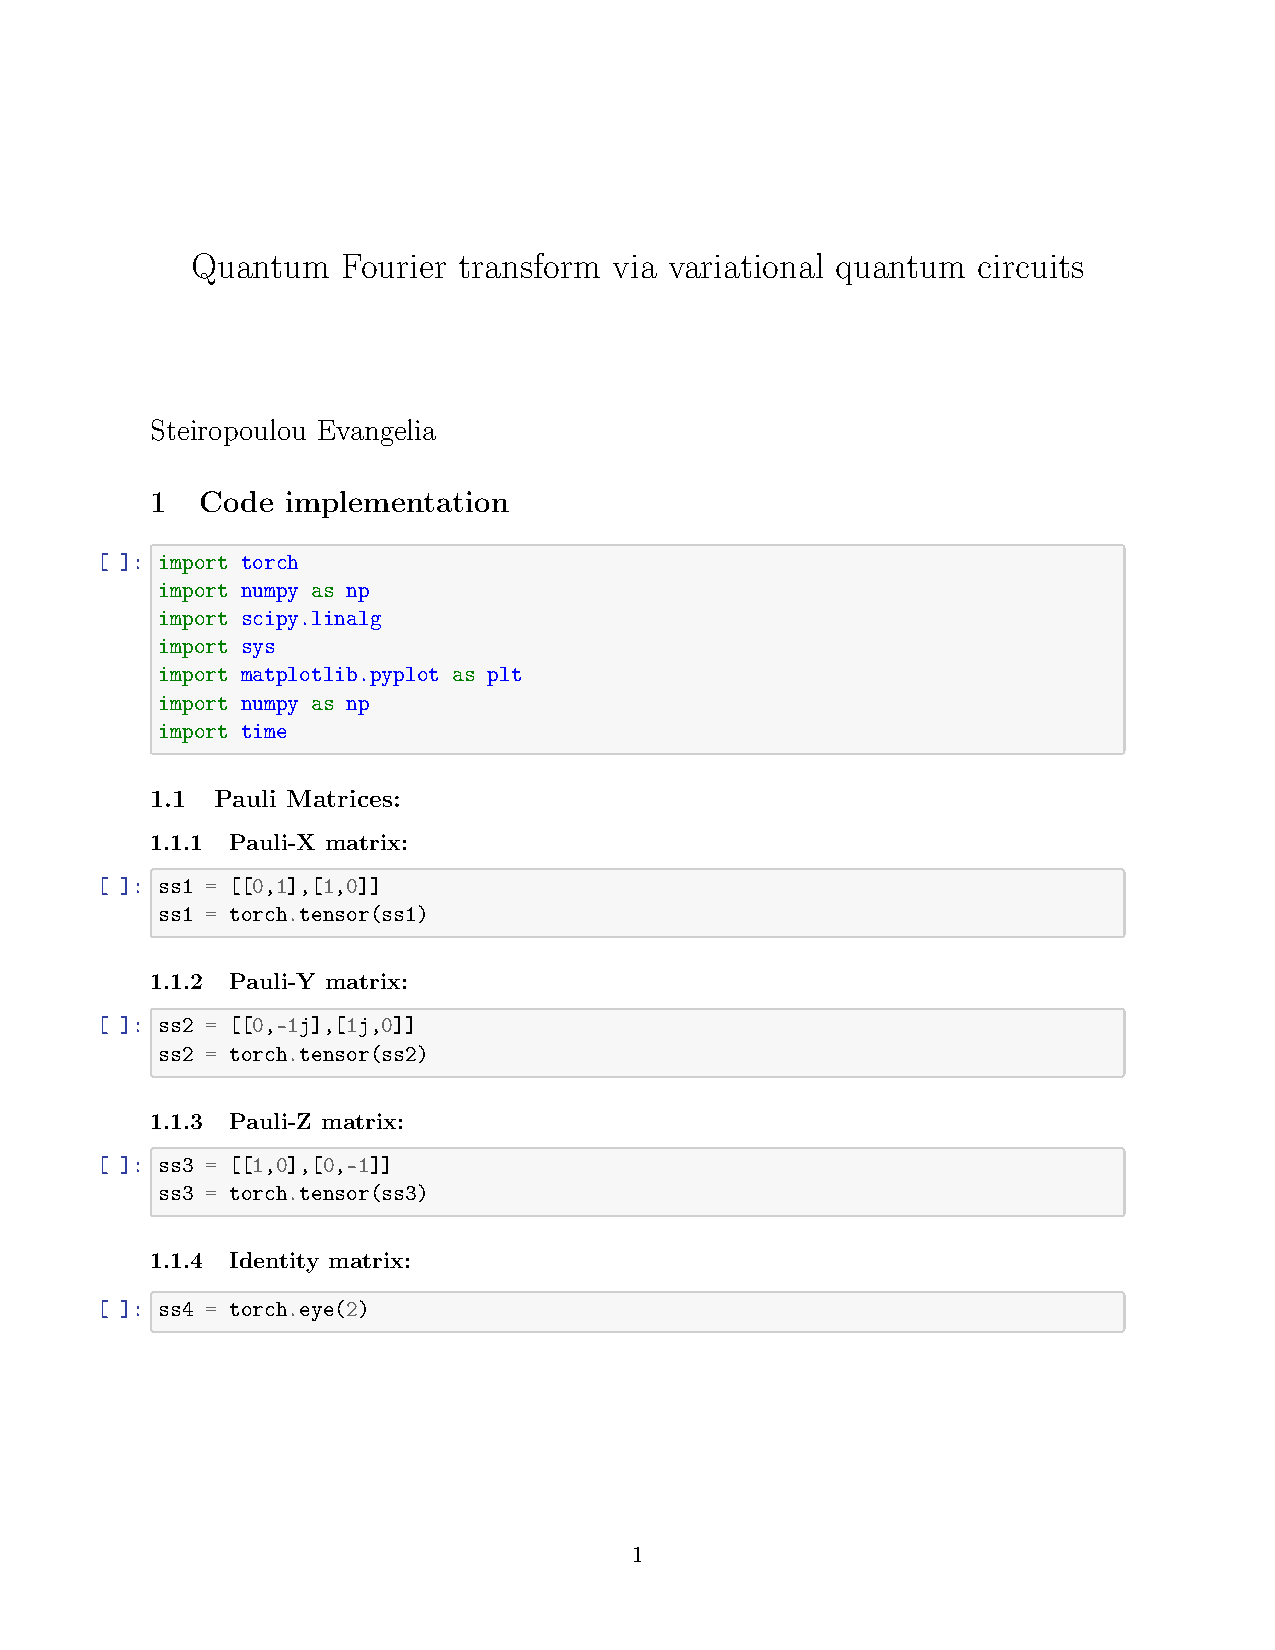
\includepdf[pages=-]{functions.pdf}

\printglossary


% manually include the bibliography
\bibliographystyle{plain}
\bibliography{references}

\begin{thebibliography}{99}                                     \footnotesize{}{
\bibitem{paper}Khatri, S., LaRose, R., Poremba, A., Cincio, L., Sornborger, A. \& Coles, P. Quantum-assisted quantum compiling. {\em Quantum}. \textbf{3} pp. 140 (2019)
\bibitem{niel}Nielsen, M. \& Chuang, I. Quantum computation and quantum information. (Cambridge university press,2010)
\bibitem{qubit}https://www.quantum-inspire.com/kbase/what-is-a-qubit/
\bibitem{polarized}https://arstechnica.com/science/2010/01/a-tale-of-two-qubits-how-quantum-computers-work/
\bibitem{electron}https://www.techtarget.com/whatis/definition/qubit
\bibitem{qudit}Wang, Y., Hu, Z., Sanders, B. \& Kais, S. Qudits and high-dimensional quantum computing. {\em Frontiers In Physics}. \textbf{8} pp. 589504 (2020)
\bibitem{hidary}Hidary, J. \& Hidary, J. Quantum computing: an applied approach. (Springer,2019)
\bibitem{kockum2014quantum}Kockum, A. Quantum optics with artificial atoms. (Chalmers Tekniska Hogskola (Sweden),2014)
\bibitem{microwave}Gaebler, J., Tan, T., Lin, Y., Wan, Y., Bowler, R., Keith, A., Glancy, S., Coakley, K., Knill, E., Leibfried, D. \& Others High-fidelity universal gate set for be 9+ ion qubits. {\em Physical Review Letters}. \textbf{117}, 060505 (2016)
\bibitem{ghz}Mermin, N. What's wrong with these elements of reality?. {\em Physics Today}. \textbf{43}, 9-11 (1990)
\bibitem{ibm}https://quantum-computing.ibm.com/composer/files
\bibitem{ghz_ibm}https://quantum-computing.ibm.com/composer/docs/iqx/guide/entanglement
\bibitem{vqc}Kimura, T., Shiba, K., Chen, C., Sogabe, M., Sakamoto, K. \& Sogabe, T. Variational quantum circuit-based reinforcement learning for POMDP and experimental implementation. {\em Mathematical Problems In Engineering}. \textbf{2021} pp. 1-11 (2021)
\bibitem{vqc2}Qi, J., Yang, C., Chen, P. \& Hsieh, M. Theoretical error performance analysis for variational quantum circuit based functional regression. {\em Npj Quantum Information}. \textbf{9}, 4 (2023)
\bibitem{vqc_arch}Du, Y., Huang, T., You, S., Hsieh, M. \& Tao, D. Quantum circuit architecture search for variational quantum algorithms. {\em Npj Quantum Information}. \textbf{8}, 62 (2022)
\bibitem{vqa}Cerezo, M., Arrasmith, A., Babbush, R., Benjamin, S., Endo, S., Fujii, K., McClean, J., Mitarai, K., Yuan, X., Cincio, L. \& Others Variational quantum algorithms. {\em Nature Reviews Physics}. \textbf{3}, 625-644 (2021)
\bibitem{limitations}De Palma, G., Marvian, M., Rouzé, C. \& França, D. Limitations of variational quantum algorithms: a quantum optimal transport approach. {\em PRX Quantum}. \textbf{4}, 010309 (2023)
\bibitem{gradient}Ruder, S. An overview of gradient descent optimization algorithms. {\em ArXiv Preprint ArXiv:1609.04747}. (2016)
\bibitem{gd}Mahanta, J. Keep it simple! How to understand Gradient Descent algorithm.  (2017)
\bibitem{supervised}Schuld, M. \& Petruccione, F. Supervised learning with quantum computers. (Springer,2018)
\bibitem{cphase}Stancil, D. \& Byrd, G. Principles of superconducting quantum computers. (John Wiley & Sons,2022)
}


\end{thebibliography}

\end{document}


\backmatter

% abbreviations table
\abbreviations
\begin{center}
	\renewcommand{\arraystretch}{1.5}
	\begin{longtable}{ l @{\qquad} l }
	\toprule
	RDF    & Resource Description Framework \\
	SPARQL & SPARQL Protocol and RDF Query Language \\
	OWL    & Web Ontology Language \\
	OGC    & Open Geospatial Consortium \\
	\bottomrule
	\end{longtable}
\end{center}

%appendix
\begin{appendix}
% mark the beginning of the appendix
\appendixstartedtrue

% add appendix line to ToC
\phantomchapter
\addcontentsline{toc}{chapter}{APPENDICES}

\chapter{FIRST APPENDIX}
\chapter{SECOND APPENDIX}
\chapter{THIRD APPENDIX}
\end{appendix}

% manually include the bibliography
\bibliographystyle{plain}
\bibliography{references}
% include it also in ToC (do sth on your own)
\addcontentsline{toc}{chapter}{REFERENCES}
